\documentclass[12pt]{article}
\usepackage[top=1in, bottom=1in, right=1in, left=1in]{geometry}
\usepackage{setspace}
\usepackage{graphicx}
\usepackage{setspace}
\usepackage{parskip}
\usepackage{url}

\title{\vspace{2.8in}Excepted Appointments and Presidential Unilateral Power}
\date{May 9, 2016}


%\usepackage{Sweave}
\begin{document}
%\Sconcordance{concordance:ExceptedAppointmentsUnilateralPowersApril21.tex:ExceptedAppointmentsUnilateralPowersApril21.Rnw:%
1 13 1 1 0 381 1}

\pagenumbering{gobble}
\maketitle
\parindent=0.5in
\parskip=0.01in
\doublespacing

\newpage
\noindent \textbf{Abstract:}

Though increasing scholarly attention has been devoted to unilateralism in recent years, the president's appointment power has largely been overlooked as a form of unilateral presidential authority. I argue that presidents use Schedule C appointments, which are excepted both from advice and consent and competitive hiring processes, when ideological conflict within the Senate is high. I find support for this hypothesis using OPM data on Schedule C appointees from 1998-2013. In sum, this study shows that excepted appointments are an important yet understudied tool in the president's unilateral policy toolbox. 

\newpage
\pagenumbering{arabic}

Over the past several decades, few topics in political science have garnered more attention than congressional gridlock. Scholars and journalists have often blamed partisan conflict within Congress for low congressional approval ratings (Binder 2003), understaffed courts and agencies (Binder and Maltzman 2009; Viser 2013), and an inability to act on key issues (Weisman 2013) or simply run the day-to-day operations of the government (Helderman 2011). Just within the Senate, critics have long blamed the filibuster for fueling obstructionist tendencies and holding up meaningful reforms (Binder and Smith 1997; Smith 2014). In 2013, Democrats resorted to using the nuclear option following frequent, prolonged Republican obstruction via filibuster on the president's lower-level judicial nominees. Frustration with the filibuster and its tendency to foster obstruction has been especially apparent in recent months as Republicans in the Senate have stalled on Merrick Garland's Supreme Court nomination.

Given the rise of congressional deadlock and obstructionism they face, it is unsurprising that presidents try to pursue their agendas without Congress. In light of this tendency, scholars have turned their attention to the increasing importance of unilateral authority. Indeed, unilateral power has become ``so pivotal to presidential leadership that it virtually defines what is distinctively modern about the modern presidency''(Moe and Howell 1999). However, most research on unilateral powers has focused on executive orders (Bolton and Thrower 2015; Howell 2003; Mayer 2002; Warber 2006). A more recent body of research incorporates other forms of unilateral action, such as memoranda (Lowande 2014) and signing statements (Kelley and Marshall 2009). However, the president's appointment authority has largely been ignored as a form of unilateral power (but see Lewis 2005). Because the most visible appointments require the president to work \textit{with} the Senate, it is easy to overlook the appointment power as a form of unilateral action. However, more than two-thirds of the president's available political appointees are not subject to Senate confirmation but nonetheless perform important functions within the government (Government Accountability Office 2012).

I argue that because they are chosen by the president without the Senate's advice and consent, excepted appointees are an important and versatile unilateral tool.\footnote{Excepted appointees, as I discuss in greater detail below, are appointees who do not go through traditional competitive hiring processes. With the exception of advice and consent or PAS appointees, excepted appointees are also exempt from Senate confirmation.} Though they lack the glamour and intrigue (as well as some of the political clout) of their Senate-confirmed counterparts, excepted appointees allow the president to continue to staff agencies when conditions in the Senate make advice and consent more difficult. Thus, I argue that as partisan conflict within the Senate increases, presidents will increasingly utilize excepted authorities. Moreover, I argue that the versatility of excepted appointees makes them additionally useful for filling new and salient agencies, which require a large amount of staff quickly.
	
	To test the relationship between excepted appointees and partisan conflict in the Senate, I focus on one type of excepted appointment authority called Schedule C.\footnote{Schedule C appointees, as I will describe in greater detail below, are useful for testing this proposition because they are the most flexibile appointment type, so if a relationship is likely to be found, it is most probably found with Schedule C appointees.} I introduce a new dataset of all Schedule C appointments from 1998 to 2013. These data show that presidents use Schedule C appointments more frequently when conflict within the Senate is high. Through a case study of the Department of Homeland Security Headquarters, I also reveal an additional aspect of the versatility of excepted appointees, showing that President Bush utilized Schedule C appointees to fill positions quickly in a new and salient agency. In combination, these results show that Schedule C appointees offer presidents the flexibility they need to fill positions quickly with ideological allies and also provides them an important means of achieving their policy goals when conditions within the Senate make using the appointment power more difficult.

\section*{Political Control and Presidential Appointments}
In November 2014, President Obama nominated Antonio Weiss, head of investment banking for independent financial management firm Lazard, as the Undersecretary for Domestic Finance. Led by Elizabeth Warren, a number of progressive Democrats in the Senate opposed Weiss' appointment.\footnote{ These Democrats were concerned about Weiss' financial industry ties, believing he may not be willing to produce stringent enough regulations. More information can be found in this article: http://www.politico.com/story/2015/01/antonio-weiss-pulls-out-treasury-undersecretary-114191\\} To avoid a confirmation showdown, Obama withdrew the nomination and instead appointed Weiss as Counselor to the Secretary of the Treasury, a position which does not require Senate confirmation. While he may have fewer formal responsibilities as Counselor than he would have as Undersecretary, Weiss had the ability to affect policy immediately rather than risking a lengthy and potentially unsuccessful confirmation battle.\footnote{Elizabeth Warren should especially appreciate the importance of these lower-level positions because she served as an excepted Schedule C appointee under Secretary Geithner, appointed for the express purpose of creating the Consumer Financial Protection Bureau. Lewis (2011) argues that Warren was appointed as a Schedule C to specifically avoid a contentious fight in the Senate.}
	
	This episode illustrates an important aspect of excepted appointees that make them powerful weapons in the president's unilateral policy arsenal. Because excepted appointees do not undergo advice and consent nor competitive hiring processes, they are incredibly versatile. Rather than wait months for appointments to be confirmed and risk potential embarrassment if they are not, presidents can appoint officials who will pursue their agendas immediately. The Weiss story illustrates the difficulty presidents face when nominees are blocked by minorities in the Senate. Presidents need not necessarily circumvent a hostile Congress with nominees a majority of members dislike, rather, presidents can utilize excepted authorities to continue to staff agencies when conditions within the Senate make confirmation difficult. In addition to the difficulties caused by confirmation delays, there may be instances in which positions must be filled quickly in order to fulfill essential tasks in an agency. New agencies related to the president's agenda need the capacity to act, sometimes without waiting for the confirmation process or competitive processes to occur. 

	Despite the usefulness of excepted appointments that the Weiss case illustrates, relatively few studies have included, much less focused on them (but see Hollibaugh et al. 2014; Lewis 2008; Lewis and Waterman 2013). This is surprising given that presidents care about how agencies execute policy and frequently use staffing to enhance their political positions (Lewis 2008; Moe 1985). For example, Lewis (2008, 2011) shows that presidents bolster their administrative control by increasing the number of appointments available to them and expanding appointment power in key management positions. Excepted appointments, which largely fly under the radar of congressional and media oversight, seem ripe for such political purposes. However, the relative dearth of scholarly interest on such appointments is likely because their invisibility seems to suggest they are unimportant to the president.
	
	Evidence suggests that presidents think carefully about hiring decisions and significant work is dedicated to unearthing this process (e.g. Hollibaugh et al. 2014; Lewis and Waterman 2013; Patterson 2008; Patterson and Pfiffner 2001; Tolchin and Tolchin 2010). For example, much scholarly work is devoted to the president's tradeoff between competent ``experts" and political loyalists (e.g. Heclo 1977; Hollibaugh et al. 2014; Lewis 2008; Moe 1985; Parsneau 2013). Additional work considers presidential patronage (Lewis 2008; Hollibaugh et al. 2014) and the politicization of presidential appointments (e.g., Burke 1992; Hart 1995; Heclo 1975; Lewis 2005, 2008; Wayne et al. 1979). Presidents care about all of these staffing decisions---whether at the top of an agency or at the mid and lower levels---because they recognize how vital staffing is to pursuing their agendas. In an interview, President Ford argued, ``if he [the president] cannot reach into the bowels of a department his decisions way up at the top will seldom be adequately implemented out in the grass roots" (Lewis 2008, 57). Thus, despite the seeming obscurity of excepted appointments, presidents do care about who fills these roles. Studying these unique and relatively invisible appointees provides important insight not just into excepted appointees as a form of unilateral authority but also as an important tool for managing the bureaucracy, especially when presidents face the perils of advice and consent. 
	
%Moreover, as Lewis (2008) admits, appointees appointed for patronage reasons may also be appointed for other reasons, such as their ideological alignment with the president, and having a patronage component to an appointment does not mean that appointee is unable to affect policy. 

%Presidents use higher-level appointees to help carry out policies on their agenda, but they also utilize excepted appointees even though they are less senior than advice and consent (PAS) appointees.\footnote{As I mention in greater detail in later sections, excepted service appointments are technically those individuals who are not appointed through the competitive hiring process. However, in practice, OPM does not refer to all employees exempt from competitive hiring as "excepted." Senate-confirmed appointees (which are excepted from the competitive service) carry the distinction ``PAS." What OPM refers to as excepted service positions are excepted both from the competitive processes and advice and consent, and this is how I choose to use the term.} Lower level appointees are often responsible for making important policy decisions or carrying out vital agency tasks. Without these lower level appointees, it may be impossible to enact the president's agenda.  Despite their usefulness to the president, lower-level appointees, and especially those who do not face Senate confirmation, generally have been overlooked in bureaucracy scholarship.
	
%While the former may attempt to shift policy closer to their own view points and away from the president's (Moe 1985), the latter may lack the skill to execute policy well or efficiently (e.g. Lewis 2005; Gilmour and Lewis 2006; Heclo 1975, 1977).\footnote{Apart from ideology and competence, the president also considers patronage when making hiring decisions (). For example, Hollibaugh et al. (2014) find that presidents place patronage appointees in agencies on the president's agenda but where they have little ability to affect policy.} Because different appointment types have different uses for presidents, they must decide how and where to best utilize them. One body of literature explores this decisionmaking process (). Scholars have been particularly concerned with a tendency for the president to ``politicize" the bureaucracy---that is, use appointees selected based on their ties to the party rather than expertise. (). While competence still plays a role, ideology is undeniably a part of the president's attempts to gain administrative control. Because they worry that appointees selected on competence will not support them ideologically, presidents are continually trying to use their appointees to control more than just the leadership of the bureaucracy (Lewis 2008).
	
\subsection*{Presidential Staffing and Political Polarization in the Senate}

Given the difficulties of the advice and consent process, it is easy to imagine why presidents need flexibility. Delay and failure are the two most obvious of many confirmation troubles and those problems have only worsened in recent years. The length of time to confirmation has increased substantially since the 1980s (O'Connell 2015). Obama's nominees waited twice as long to be confirmed as Reagan's. Moreover, over 25 percent of presidential nominations failed since the 1980s with greater failure rates for Bush and Obama than their predecessors. Reagan appointed 86 percent of his top officials in his first year, but Obama could not complete two-thirds (Pfiffner 2015).\footnote{Wait times likely started increasing even before the Reagan presidency. The average JFK appointee waited only 2.5 months to be confirmed by the Senate while the average George W. Bush appointee waited nine months (Pfiffner 2015).} 

Partisan conflict within the Senate seems to exacerbate these problems (McCarty and Razaghian 1999). At times, a minority in the Senate may oppose the president's nominees for political reasons or the Senate may be too polarized to agree on a nominee. Indeed, senators work to strategically delay nominations by, for instance, refusing to hold hearings on or vote to confirm a nominee for so long that the president is eventually forced to withdraw the nomination (Bond et al 2009; Ostrander forthcoming). Moreover, partisan senators may use nominees as bargaining chips in political conflicts. Kenneth Kopocis, a nominee for the EPA, had waited more than 1,000 days because Republicans did not support one of the EPA's proposed rules and used his nomination as leverage to revoke it (Eilperin 2014). The nuclear option implemented in 2013 did not seem to solve the problem. While these filibuster reforms decreased wait times for judicial nominees, they increased wait times for other nominees (O'Connell 2015). 

Lengthy confirmation ordeals can severely hinder the president's agenda (Lewis 2011; McCarty and Razaghian 1999). While confirmation rates are similar to other presidents, Obama's nominees have waited an average of 265 days to be confirmed (Eilperin 2014). Describing the confirmation process as ``a living purgatory," the chief executive of the Partnership for Public Service explained that the process has dissuaded some of the very best candidates from applying. If candidates are not from the DC area already, the cost of the confirmation process for nominees is considerable. One law professor from Indiana rented a home in Maryland and commuted back and forth at her own expense, waiting 14 months for a confirmation vote which never occurred. She finally had her nomination withdrawn. Because of these considerable expenses, long waits dissuade less wealthy or geopgraphical diverse indiviuals from taking advice and consent positions. This limits the president's options and deters talented people from working in the administration (Eilperin 2014). Alternatively, the excepted service allows the president to select talented individuals who are unwilling or unable to undergo advice and consent.\footnote{The excepted service is not necessarily used as an alternative for all advice and consent nominees as it was with Weiss.} Lengthy confirmation processes can be especially damaging late in a presidency, when the failure to confirm a president's nominees can derail the agenda that nominee hoped to pursue in office.

Presidents do not want their agendas to be held up by a lack of personnel, and if faced with high levels of partisan conflict in the Senate, we would expect presidents to find other means to staff their agencies just as they find other means to make policy. Excepted appointments give presidents just this ability. The increasing failures and confirmation delays described above mean an increase in the time to filling vacancies, which happen often given the relatively short amount of time appointees stay in their positions (O'Connell 2008; Pfiffner 2015). Top positions in cabinet and executive agencies are vacant or filled by an acting official 15 to 25 percent of the time in recent years (O'Connell 2008). Missing leadership in agencies can lead to delays in the president's regulatory agenda. However, excepted appointees can help ease this burden. While not a perfect substitute for missing advice and consent officials, excepted appointees can help keep an agency on task in their absence. Indeed, advice and consent vacancies leave room for excepted appointees to exercise greater influence over policy than they normally would (O'Connell 2010).\footnote{Conversations with Schedule C appointees confirm this notion. Two individuals suggested that when major vacancies occured among advice and consent officials they took on a more active role in their agency.}

Given the predicament presidents face with regard to staffing in recent years, it is important to consider the conditions under which they will resort to using excepted appointees to augment the advice and consent process.\footnote{As I describe in the next section, excepted appointments are not perfect substitutes for advice and consent appointees. Excepted appointees are often advisors and rarely have the same influence and background as advice and consent appointees. However, they tend to take on greater roles in the absence of advice and consent appointees and they can help to steer the agency toward the president when acting officials, who are often career appointees, take over.} While some evidence has indicated that unilateral actions like executive orders and memoranda may occur more often in unified government than divided government (Howell 2003; Lowande 2014), theoretical and empirical evidence indicates conditions within Congress may be just as (if not more) important than the relationship between the president and Congress for inducing unilateral activity (Bolton and Thrower 2015; Howell 2003). Consistent with these findings, I argue that a higher level of conflict within the Senate increases the likelihood that the president will utilize Schedule C appointees.\footnote{It is important to reiterate that greater ideological distances between the president and the Senate will not necessarily increase the use of Schedule C appointments. Rather than a method for confirming nominees the majority of senators dislike, Schedule C and other excepted authorities allow the president to act when conflict within the Senate makes confirmation more difficult.} 

\textit{H1: Presidents will utilize greater (fewer) numbers of Schedule C appointments when conflict within the Senate is high (low).}

\section*{Excepted Service and the Larger Appointment System}

	It is useful to understand how excepted appointments fit in the larger appointment system. While most scholarship tends to focus on traditional advice and consent appointments, most jobs in the bureaucracy are filled through a competitive process open to the public just as industry jobs are filled. Excepted service positions are technically those appointments that have been excepted from the competitive hiring process. Positions like Schedule C or Senior Executive Service (SES) are also exempt from advice and consent.\footnote{Some excepted service appointments are reserved for positions for which the Office of Personnel Management (OPM) does not or cannot provide a test or standard (professionals such as lawyers are one example). Other excepted service appointments are reserved for those with disabilities or are set aside for interns. These appointments, like competitive service appointments, are largely used to complete the day-to-day operations of the government.}	Unlike many other excepted positions, Schedule C appointments are positions excepted for political reasons. OPM describes Schedule C appointments as those positions of a ``confidential" or ``policy-determining nature," for which it is important the employee shares the president's vision for the agency. Figure 1 puts agency hierarchy into perspective for the Department of Agriculture, showing one page of the Plum Book (U.S. House of Representatives 2012, 11).\footnote{The Plum Book is a government publication released once every four years by Congress. It began in the Eisenhower administration for the same reasons that he created Schedule C: because he did not have enough information about the bureaucracy. The Plum Book lists appointments available for the president to make. He can later add Schedule C positions not listed in the Plum Book.} Senate-confirmed PAS appointees occupy top positions. NA appointees (Non-career appointees, like SES) occupy many high positions, but Schedule Cs often occupy the positions immediately below these Senior Executive Service appointees.\footnote{The TA appointment is a temporary appointment.}
	
PAS appointees fill the senior-most positions in the Department of Agriculture. The Secretary of Agriculture, of course, is responsible for communicating with the president and dictating policy within the department. The Deputy Secretary works directly with the secretary to fulfill the policy goals for the agency and communicate them with the various sub-departments. The Department of Agriculture covers a vast array of policy areas---domestic and international trade and agriculture, food safety, nutrition, rural development, and more. Because of this policy breadth, the Department has many Deputy Undersecretaries serving in these various sub-departments. These individuals are typically non-career SES appointees---senior officials who are also excepted from both advice and consent and the competitive civil service. These deputy undersecretaries are tasked with advising the more senior PAS staff on their individual policy areas. Schedule C appointees provide a wide array of services within agencies. Some serve as scheduling assistants and speech writers; others serve as more important policy advisors. Special Assistants, for example, typically advise the deputy undersecretary on specific policy areas, but they may be asked to fill whatever current needs in the department may be. Schedule C chiefs of staff within sub-departments fill somewhat more important roles. They may brief deputy undersecretaries, control their schedules, fill in for them in their absence, approve rules created by career staff, and resolve disputes between employees. 
	
\begin{center}[Figure 1 About Here]	\end{center}

	President Eisenhower created Schedule C appointments when he first reached office. According to Gailmard and Patty (2012), Eisenhower instituted Schedule C because he was faced with the political realities of being the first Republican to win the presidency in twenty years (leaving him with few trusted advisors) and because the post-World War II era left him with an expansive administrative state, which reached further into the economy and society than had previously been conceived. Schedule C was designed to exist between other classes of appointments---appointees beholden directly to the president, but who did not undergo advice and consent or competitive service processes. Today, Schedule C appointees make up about 15 percent of the president's available appointments in the Plum Book and 37 percent of the president's total political appointments (Government Accountability Office 2012).
	
	Schedule C positions are created uniquely for each employee. When the administration wishes to hire someone via Schedule C, it files paperwork with OPM detailing the responsibilities of the position to justify a particular pay grade and describes its role within the home agency. When the Schedule C is fired or quits, the position is dissolved. If the administration wishes to hire another person to fulfill the role, it must file the paperwork to create the position anew. In other words, Schedule C appointees are not filling a statutory position; they are filling the administration's current needs.	
	
	Though Schedule C positions are not as prestigious as Senate-confirmed appointments, they can still have an impact on policy. Lewis and Waterman (2013) describe a Department of Justice investigation, which found that a Senior Executive Service and former Schedule C appointee, Monica Goodling, was involved in hiring, firing, and promoting civil servants on the basis of political views. Similar lower level appointees engaged in ``bullying career staff, censoring government reports, and leaking internal documents to outside groups in order to pursue the administration's policy and political goals" (Lewis and Waterman 2013, pg. 36). Lewis and Waterman go on to note of Goodling that despite her ``low" status, she ``initiated a series of crucial, politically and legally questionable decisions" (pg. 36). 
	
\section*{Data: Schedule C Appointees 1998-2013}

The federal employment and accessions data come from the FedScope tool through the Office of Personnel Management.\footnote{OPM refers to Fedscope as the Enterprise Human Resources Integration-Statistical Data Mart (EHRI-SDM).} From the FedScope tool, I collected static data on employment statistics for September 1998-2013. These data are a picture-in-time of employment in federal agencies, representing the total employment to each included agency for September of the given year. Over the period, there were 692 agency units, some of which were created or disbanded during the time period. These are counted based on which agencies have unique agency codes (given by OPM) in the data.\footnote{Most cabinet agencies provide data below the department level. For example, the Department of Defense is massive and includes sub-departments for the Army, Navy, Air Force, and general DOD and within these departments there are unique agencies bearing the department prefix. For example, the Air Force bears the prefix ``AF" so the Air Force Operational Test and Evaluation Center is labeled ``AF03." The State Department and Department of Energy do not provide data at the sub-level. Most independent agencies (e.g. EPA or SEC) do not provide data below the overall agency level, although a few do. The FedScope database is fairly comprehensive. However, it does exclude intelligence agencies and the U.S. Postal Service in its reporting, so it is not a complete representation of every federal employee. The State Department also does not report on Foreign Service Personnel.}

Figure 2 displays the number of Schedule C appointees from 1998-2013 and the number of Schedule C accessions (new hires and transfers) from 2005-2013. Unfortunately, FedScope does not currently report accessions data prior to FY2005. 

\begin{center}[Figure 2 About Here]\end{center}

Overall, President Bush used Schedule Cs more frequently than either Clinton or Obama. In general, the number of Schedule Cs decreases and then increases when a new president takes over. As is visible, the number of accessions in 2009, when Obama takes office, is extraordinarily high---almost matching the total number of appointees in that year. While there is always some turnover during a presidential transition, this turnover is higher for political positions. The number of Schedule C accessions as a percentage of Schedule C employees is typically between 20 and 35 percent. For the Obama transition, the number of accessions as percentage of employees was over 96 percent. This suggests that 96 percent of all appointees serving in 2009 were hired under Obama and were not holdovers from the Bush administration.

The outcome variable I use for the model is the number of Schedule C appointments in an agency in a given year. A histogram of the dependent variable is available in the appendix.\footnote{Given the large number of observations with a value of 0, I also ran the model as a zero-inflated negative binomial regression. The results are virtually identical--all signs and significance levels are the same as reported in the next section and the effect sizes are similar.} The number of appointees in an agency-year ranges from 0 to 211. The mean number of appointees is 21.78 with a standard deviation of 35.7.

There is wide variation in the number of Schedule C appointees both within and across agencies over time. Figure 3 shows the pattern of Schedule C appointees in six selected agencies from 1998 through 2013. As is visible, the Department of Agriculture and the State Department have a very large number of Schedule C appointees relative to the mean. Both of these departments had relatively stable levels of Schedule C appointees through the Bush and Obama administrations. The Department of Agriculture saw a decrease in appointees from Clinton to Bush while the Department of State experienced the opposite pattern. The EPA and Small Business Administration (in the second row of plots) had moderately larger numbers of Schedule C appointees than the average agency. The EPA saw a large increase in appointees under President Bush (reaching a high of 40 appointees) but higher levels under Obama than under Clinton (with a low of seven appointees). The Small Business Administration also experienced wide variation in its level of Schedule C appointees ranging from 16 to 45 appointees over the period. The Office of Personnel Management and Consumer Product Safety Commission had a moderately lower number of Schedule C appointees relative to the mean agency. However, these agencies still experienced variation. OPM had between 11 and 24 appointees over the period with higher levels between 2002 and 2005. The Consumer Product Safety Commission had between three and 16 appointees, hitting a low in Bush's second term and a high in the Obama administration.  

\begin{center}[Figure 3 About Here]\end{center}

\subsection*{Key Variables:}

\noindent \textbf{Within-Senate Conflict:} This variable is measured using the absolute common space distance between the median member of both parties in the Senate. This is a departure from some previous literature, where divided government is frequently an independent variable.\footnote{I alternatively specified the model using an indicator for divided government, which was also positive and significant. Available in the appendix.} The distance between party medians has ranged from 0.72 to 0.98 between 1998 and 2000, with an average distance of .810. The smallest distance between party medians occurred in 1999, with the largest distance occurring in 2013. 

\subsection*{Controls:}
I control for several potential confounding factors, including agency size, which is measured as the total level of employment (in thousands) in an agency as reported by Fedscope. I expect agency size to be positively related to numbers of Schedule Cs because these agencies have more employees overall. I also include an indicator for the first (2001 and 2009) and last (2000 and 20008) years of a presidency because overall levels of employment are lower just before and after presidential transitions. I also include a measure for the distance between the president and the 60th senator and indicators for each president. Based on the figure, President Bush appears to have used a higher number of Schedule Cs than his Democratic colleagues, so I expect indicators for both Bush and Clinton to be signed negatively. I also include a control for the absolute ideological distance between an agency and the president. Agency ideology is measured using common space ideal points created by Chen and Johnson (2015). The president's ideal point comes from the Poole and Rosenthal common space measures. The agency ideology scores are unique for each term from Clinton through Obama's first term based on federal employee campaign contributions. Importantly, these scores are scaled in common space, allowing for a comparison between the ideology of agencies and the president. Thus, the ideology measure is simply the absolute distance between an agency and the president for a given year. For example, observations in 1998, 1999, and 2000 are based on Chen and Johnson's ideal point estimates for Clinton's second term and Poole and Rosenthal's estimates for Clinton. Similarly, 2001-2004 is based on the ideal point estimates for Bush's first term, 2005-2008 on his second and so on.\footnote{Chen and Johnson did not provide estimates for 2013, so I used the estimates from Obama's first term. Chen and Johnson report 79 agencies scores. Due to differences in data coverage, the models cover 64 agencies and departments. Most of this discrepancy comes from the fact that departments are rolled into one. Whereas Fedscope includes all the sub-units of a department, those who estimate agency ideology typically estimate it for the departments as a whole. For this reason, I collapsed the appointment data for all departmental sub-units into a single number for the whole department.}

\section*{Results}
The results of the negative binomial regression model with standard errors clustered on agency are reported in Table 1.\footnote{I also ran the model as a zero-inflated negative binomial regression. The results are virtually identical--all signs and significance levels are the same as reported and the effect sizes are similar. Because there are multiple observations on each agency and these observations are likely correlated with each other, clustering on the agency allows us to obtain a more reasonable estimate of the standard errors.} The results suggest support for the hypothesis. Schedule C appointees are utilized much more frequently as the distance between party medians in the Senate increases.\footnote{Results using divided government instead of distance between party medians is visible in the appendix.} On average, Obama and Clinton used fewer Schedule Cs than did President Bush, which is consistent with the plot of Schedule Cs in the previous section. Larger agencies receive greater number of Schedule Cs on average, suggesting that agencies with higher levels of overall employment also see higher levels of Schedule C appointees. The first year of a presidency also has statistically lower levels of Schedule Cs. While Schedule Cs are flexible and can be appointed quickly, it is not always possible to fill every position in the first year, especially after losing virtually all previous Schedule Cs during a transition. The last year of a presidency does have a negative sign, indicating relatively lower levels in preparation for the transition, but the result was not statistically significant. 

\begin{center}[Table 1 About Here]\end{center}

The distance between the president and the 60th senator is negative and significant, indicating that greater distances between the president and the 60th senator are associated with fewer Schedule C appointees in agencies. At first glance, this would seem to run counter to the idea that the president can use Schedule C appointees as a form of unilateral power. After all, we might expect conflict between the Senate and the president to result in the president utilizing Schedule C authority more frequently. However, while the Senate does not have a say on individual excepted appointments, Congress does control the Schedule C authority as a whole. In the 1980s and 1990s, presidents had used Schedule C authority to create details to the White House within individual departments and agencies.\footnote{This was especially problematic because the Schedule C appointees were being billed to agencies rather than the White House.} The Government Accountability Office released several reports urging OPM to establish guidelines that would prohibit this practice. OPM refused to do so and Congress ultimately passed a law prohibiting the use of Schedule Cs as White House details (Government Accountability Office 1992). This story illustrates that presidents, while given considerable leeway in the use of Schedule C appointees, must nonetheless be careful not to go too far. Much as presidents must take care not to overstep their bounds with executive orders lest they be curbed by Congress or the courts, presidents also must take care not to abuse their Schedule C authorities. This indicates presidents need not necessarily circumvent the Senate by appointing individuals a majority of members would oppose. Rather, Schedule C authority allows the president to act when conflict within the Senate makes staffing more difficult.

The distance between the agency and the president shows a negative and significant coefficient, suggesting that presidents tend to use Schedule C appointees more frequently in ideologically similar agencies. Lewis (2008) suggests that Schedule C appointees may be used more frequently in ideologically proximate agencies because they are typically used for patronage. However, evidence suggests agencies vary in their policy views and willingness to follow the president's directives (Aberbach and Rockman 1976, 1995, 2000; Bertelli and Grose 2009; Clinton and Lewis 2008; Clinton et al. 2012; Hollibaugh et al. 2014). Because of this, it is not clear ex ante which strategy the president will use to staff agencies---bolstering allies in ideologically similar agencies or offsetting enemies in ideologically distant ones. Thus, it may be that Schedule C appointees are used more frequently in ideologically proximate agencies because the president wishes to support the work of his ideological allies rather than just stacking agencies with patronage jobs. Rather, this ideology result may be due to the postion Schedule C appointees occupy within the government.

Schedule C appointees, unlike other types of excepted appointments, are uniquely situated within the personnel system. Schedule C appointees must have a Senate-confirmed (PAS) appointee, a career or non-career Senior Executive Service (SES) appointee or fellow Schedule C appointee as their immediate supervisor (House of Representatives 2012, 203). Schedule Cs may serve in a variety of different roles, but they tend to be advisors who do not have the authority to decide policy directions on their own. Rather, they work for and advise the people who do have the ability to decide an agency's direction. Presidents would prefer to be able to move wayward, ideologically distant agencies closer to their own ideal points, but they must use other appointment types to accomplish this goal. It makes sense, then, that presidents would utilize Schedule C appointees in agencies in which their advice is more likely to be heeded: ideologically similar agencies. In other words, presidents realize that giving valuable political advisors to agency decisionmakers inclined to listen to their advice is more profitable than assigning them at random or worse, to agencies with decisionmakers who actively disregard them. Importantly, appointees both to PAS and non-career SES are at least partly chosen by someone other than the president---the Senate has a say on who gets appointed to PAS appointments and competitive service processes make career SES staff less politicized. Schedule C authority allows presidents to cultivate advisors absent these limitations who can influence the influencers, and presidents are unlikely to waste this opportunity.

The main results for within-Senate conflict are visualized in Figure 4. These plots show the predicted number of Schedule Cs for all values within the range of the variable of interest for each president, holding all other variables at their mean or default values. The shaded regions are the 95 percent confidence intervals around the prediction. Bush and Clinton's confidence intervals overlap, showing that for the within-Senate conlict variable, the two presidents were not significantly different from each other. However, Bush utilized statistically larger numbers of Schedule C appointees than Obama (and for certain ranges of the data, Clinton), all other variables constant.\footnote{These plots are based on the predicted values obtained when first or last year of the presidency takes a value of zero.} To put these results into more substantive terms, an agency in the Bush administration could expect to receive 44 appointments with all variables set to their mean or reference levels. A one standard deviation increase in the conflict within the Senate would result in an agency going from 44 to 58 Schedule C appointees.

\begin{center}[Figure 4 About Here]\end{center}

Importantly, this result indicates that presidents do seem to consider the conditions within the Senate when making staffing decisions. When Congress is plagued by greater levels of polarization (and greater gridlock), the president can continue to staff agencies through other means by increasing the number of Schedule C appointees. Considering the increasing levels of congressional polarization and worsening conditions for achieving legislation that modern presidents face, Schedule Cs may become increasingly important to the president's agenda as time goes on. Given unfavorable conditions for staffing in the Senate, increasing wait times for advice and consent, and a shrinking pool of talent for traditional appointees because of these problems, the ease with which Schedule Cs can be appointed certainly increases their attractiveness to the president. This finding also suggests that just as the president uses executive orders, national security directions, and memoranda in lieu of legislation and executive agreements in lieu of treaties, presidents can augment the advice and consent process with the use of excepted appointees.

\section*{Homeland Security Headquarters: A Case Study}
The results above show one way the president might utilize the versatility of Schedule C appointees. However, Schedule C authority is not limited merely to situations in which conditions in the Senate encourage the president to seek alternative staffing solutions. Indeed, flexibility can take on a variety of forms. In some instances, presidents may need to fill positions quickly for other reasons. For example, new and salient agencies require a large number of personnel quickly. The case of the Homeland Security Headquarters illustrates how the versatility of Schedule C authority can be useful to presidents even when the Senate is complicit with their wishes. 

The Department of Homeland Security was created in direct response to 9/11. While there had been calls for the creation of a Homeland Security office earlier in 2001, it was the September 11 attacks which expedited the process. Fewer than two weeks passed before President Bush selected Governor Tom Ridge to head a new Homeland Security Office. In November of 2002, DHS was officially born as a cabinet agency by act of Congress. It began operating in March 2003 (Department Homeland Security 2014). Between the creation of a brand new cabinet department and the expediency with which President Bush pushed his agenda following the September 11 attacks and into the War on Terror, it is no surprise he would need to fill positions quickly. It is also no surprise that President Bush fought for wide discretion in DHS's creation. In fact, he used the need for expediency and discretion as a justification for his attempt to create a separate personnel system for Homeland Security that would not operate with typical civil service protections. According to the \textit{Washington Post}, Bush officials argued that the September 11 attacks required changes that would ``give more discretion to managers and permit quicker deployment of workers without notifying their union representatives" (Barr 2008). Due to their flexible nature, President Bush utilized Schedule C appointees to get the Homeland Security Headquarters up and running quickly.

Twelve Schedule C appointees were placed in the Department of Homeland Security in January of 2003. Some of these appointees were travel aids, receptionists, and scheduling assistants appointed to aid the Secretary and Undersecretary of Homeland Security in their everyday needs. Bush also appointed several speechwriters and an assistant press secretary to assist with communicating the department's messages to other agencies, the Senate, and the public. Some of these early Schedule C appointees also worked as special assistants who serve as advisors to the secretary and liaisons with career staff on individual policy matters. Thus, these early Schedule Cs filled both practical and policy needs within the agency.

Figure 5 corroborates the versatility story. In 2003, over 40 percent of the Homeland Security Headquarters was staffed by Schedule C appointments.\footnote{The above descriptive statistics are reported with regard to the Department of Homeland Security as a whole. This figure is in reference to the Department of Homeland Security's headquarters as opposed to the entire set of sub-agencies within DHS.} This proportion has gradually declined ever since. In the right half of the figure we see the raw number of Schedule C appointees. The number nearly doubled from 2003 to 2004 yet the proportion of the agency employment made up by Schedule C appointees declined. This is likely because the president used Schedule C appointments to fill the department quickly, but as time went on, new hires of other appointment types came in.

\begin{center}[Figure 5 About Here]\end{center}

Importantly, these results show that presidents can and do utilize Schedule C appointees for the flexibility they provide. In 2003, conditions in the Senate were favorable for President Bush, but he nonetheless required staff quickly. The confirmation process requires significant Senate time and resources and would take an especially long time if every official needed to go through advice and consent or competitive processes. In other words, while the Senate was amenable to the president's wishes (and even completed a few advice and consent appointments quickly), it would have been impractical to use advice and consent to fill all of the nascent department's staffing needs. Because of Schedule C authority, high-level officials could receive the support they needed to implement the president's agenda throughout all levels of the department. Most importantly, the president was able to fill these positions with the people of his choosing and do so without the fanfare that typically accompanies high-profile nominations. 

\section*{Conclusion}	
When presidents reach office, they are met with the difficulty of managing an expansive bureaucratic state. They work with the Senate to fill leadership positions in hundreds of agencies, but there are thousands of political appointee positions to fill. With the increasing length of time to confirmation and increasing levels of polarization, presidents especially need the flexibility that excepted appointments afford them. The fact that we observe higher numbers of Schedule C positions as within-Senate conflict increases should come as no surprise to students of unilateral politics. As shown in Howell's theory and Bolton and Thrower's empirical results with executive orders (Howell 2003), presidents utilize unilateral actions more frequently in the presence of within-Senate conflict. 

%Schedule C positions are useful to presidents because they allow them to bypass the Senate when it faces high levels of internal conflict, but this is not their only use. Presidents need to fill positions at all levels of the bureaucracy in order to fully pursue their agendas, in part because they need lower level personnel to help implement policy. Because the president has the freedom to select the appointees of his choosing and appoint them when and where he sees fit, Schedule C appointees are an especially important tool. Schedule C appointees largely serve as advisors without signing authority of their own, so the president is more likely to utilize them where their advice is more likely to be heeded. As I have shown, presidents tend to utilize this appointment type more frequently in ideologically similar agencies.

In addition to these main findings, the case of the Department of Homeland Security headquarters corroborates the flexibility story by suggesting another potential avenue for the use of Schedule Cs. Given urgent situations, presidents can use Schedule Cs to fill positions quickly, boosting an agency's capacity to act. With a new cabinet department and President Bush emphasizing a sense of urgency, it is no surprise that Schedule C appointees quickly filled DHS headquarters' ranks initially, only for the proportion to decline as more positions were filled. Though the creation of a new agency in a salient policy area is an obvious place to look for an increase in excepted appointments, other research has indicated that absences in agency leadership often allow excepted appointees to take on larger roles within an agency.

These findings have important implications for how the president manages the executive branch. Though the president can act alone to create Schedule C positions, excepted authority need not serve as an example of nefarious presidential overreach. Rather, presidents need a way to keep agencies working when the Senate drags its heels or fails to confirm traditional appointees. In short, Schedule C appointees are a managerial response to the challenges of governing presidents share with Congress. Indeed, the president faces a tradeoff when using excepted authorities. While versatile, Schedule C appointees do not possess the same authority as their Senate-confirmed counterparts. Future theoretical work must consider the conditions under which presidents would rather bear the costs of confirmation over utilizing Schedule C appointees.

Importantly, these results indicate just how necessary it is for bureaucratic scholars to consider a wider range of appointment types in their theories of staffing. Given how many appointees are not subject to Senate approval and given that these appointees are often involved in important decisionmaking within agencies, it is surprising they have not been given more scholarly attention. Even more broadly, it shows that scholars have been relatively narrow-minded when considering presidential unilateral authority. Presidency scholars have largely focused on more obvious or tangible methods of unilateral action, but there are many ways for presidents to exert their authority. This study has offered evidence showing that excepted appointments are yet another method presidents can use to pursue their policy agendas without Congress or in spite of it. These results have merely skimmed the surface of how Schedule C appointees might be studied, however. Little is known, for example, how appointees like these might be related to tangible bureaucratic outputs such as rulemaking activity or how they are affected by transitions in agency leadership.

As Lewis and Waterman (2013) state, it is important to ``lift the veil from the president's invisible appointments." A deeper understanding of how excepted appointments fit into the broader bureaucratic system and how they are affected by the outside winds of political forces are an important step in developing a more comprehensive understanding of federal bureaucracy. This study hopes to contribute to the lifting of the veil by better understanding how these appointees can be used as an important weapon in the president's unilateral arsenal.

\newpage
\section*{References}
\singlespacing
\noindent \hangindent=0.7cm Aberbach, Joel D.,  and Bert A. Rockman. 1976. ``Clashing Beliefs withing the Executive Branch: The Nixon Administration Bureaucracy." \textit{American Political Science Review} 70(2): 456-468. 

\noindent \hangindent=0.7cm Aberbach, Joel D., and Bert A. Rockman. 1995. ``The Political Views of U.S. Senior Federal Executives, 1970-1992. \textit{Journal of Politics} 57(3): 838-52. 

\noindent \hangindent=0.7cm Aberbach, Joel D., and Bert A. Rockman. 2000. \textit{In the Web of Politics: Three Decades of the U.S. Federal Executive.} Washington, DC: Brookings Institution.

\noindent \hangindent=0.7cm Barr, Stephen. 2008. ``DHS Withdraws Bid to Curb Union Rights." \textit{Washington Post}. \url{http://www.washingtonpost.com/wp-dyn/content/article/2008/02/1/AR2008021902459.html}. Last accessed January 6, 2014.

\noindent \hangindent=0.7cm Bertelli, Anthony, and Christian Grose. 2009. ``Secretaries or Pork? A New Theory of Distributive Politics." \textit{Journal of Politics} 71(3): 926-945. 

\noindent \hangindent=0.7cm Binder, Sarah. 2003. \textit{Stalemate: Causes and Consequences of Legislative Gridlock.} Washington, DC: Brookings Institution.

\noindent \hangindent=0.7cm Binder, Sarah and Forrest Maltzman. \textit{Advice and Dissent: The Struggle to Shape the Federal Judiciary.} Washington, DC: Brookings Institution. 

\noindent \hangindent=0.7cm Binder, Sarah and Steven S. Smith. 1996. \textit{Politics or Principle: Fillibustering in the United States Senate.} Washington, DC: Brookings Institution. 

\noindent \hangindent=0.7cm Bolton, Alexander and Sharece Thrower. 2015. ``Legislative Capacity and Executive Unilateralism." \textit{American Journal of Political Science}. 

\noindent \hangindent=0.7cm Bond, Jon R., Richard Fleisher and Glen S. Krutz. 2009. ``Malign Neglect: Evidence That Delay Has Become the Primary Method of Defeating Presidential Appointments'' \textit{Congress and the Presidency} 36(3): 226-243.

\noindent \hangindent=0.7cm Burke, John P. 1992. \textit{The Institutional Presidency}. Baltimore: Johns Hopkins University Press. 

\noindent \hangindent=0.7cm Chen, Jowei and Tim Johnson. 2015. "Federal employee unionization and presidential control of the bureaucracy: Estimating and explaining ideological change in executive agencies." Journal of Theoretical Politics 27(1):151-174.

\noindent \hangindent=0.7cm Clinton, Joshua D., Anthony Bertelli, Christian Grose, David E. Lewis and David C. Nixon. 2012. ``Separated Powers in the United States." American Journal of Political Science 56(2):341-54.

\noindent \hangindent=0.7cm Clinton, Joshua D., and David E. Lewis. 2008. "Expert Opinion, Agency Characteristics, and Agency Preferences." Political Analysis 16:3-20.

\noindent \hangindent=0.7cm Eilperin, Juliet. 2014. ``Chances for Obama nominees to be confirmed are falling, even with over two years to go." \textit{Washington Post}. \url{https://www.washingtonpost.com/politics/chances-for-obama-nominees-to-be-confirmed-are-falling-even-with-over-two-years-to-go/2014/03/26/73a87b84-b107-11e3-9627-c65021d6d572_story.html}. Last accessed December 15, 2015. 

\noindent \hangindent=0.7cm Gailmard, Sean and John W. Patty. 2012. \textit{Learning While Governing.} Chicago: University of Chicago Press. 

\noindent \hangindent=0.7cm Gilmour, John B., and David E. Lewis. 2006. ``Political Appointees and the Competence of Federal Program Management." \textit{American Politics Research} 34(1):22-50. 

\noindent \hangindent=0.7cm Government Accountability Office. 1992. \textit{Personnel Practices: Schedule C and Other Details to the Executive Office of the President.} Washington, DC: Government Printing Office.

\noindent \hangindent=0.7cm Government Accountability Office. 2012. \textit{Characteristics of Presidential Appointments That Do Not Require Senate Confirmation.} Washington, DC: Government Printing Office.

\noindent \hangindent=0.7cm Hart, John. 1995. \textit{The Presidential Branch}.  New York: Chatham House.

\noindent \hangindent=0.7cm Heclo, Hugh. 1975. ``OMB and the presidency---The problem of `neutral competence.'" \textit{Public Interest} 38(Winter): 80-98.

\noindent \hangindent=0.7cm Heclo, Hugh. 1977. \textit{A Government of Strangers: Executive Politics in Washington}. Washington, DC: Brookings Institution.

\noindent \hangindent=0.7cm Helderman, Rosalind S. 2011. ``Congress struggles to fix budget gridlock as another deadline looms." \textit{Washington Post.} \url{https://www.washingtonpost.com/politics/congress-struggles-to-fix-budget-gridlock-as-another-deadline-looms/2011/10/18/gIQAKYZ6IM_story.html} Last accessed May 3, 2016. 

\noindent \hangindent=0.7cm Hollibaugh, Gary E. 2014. "Naive Cronyism and Neutral Competence: Patronage, Performance, and Policy Agreement in Executive Appointments" \textit{Journal of Public Administration Research and Theory} 25(2): 341-372. 

\noindent \hangindent=0.7cm Hollibaugh Jr., Gary E., Gabe Horton, and David E. Lewis. 2014. ``Presidents and Patronage." \textit{American Journal of Political Science.} 58(4): 1024-1042.

\noindent \hangindent=0.7cm Howell, William G. \textit{Power Without Persuasion.} Princeton, NJ: Princeton University Press.

\noindent \hangindent=0.7cm Kelley, Christopher and Marshall, Bryan. W. 2009. ``Assessing Presidential Power: Signing Statements and Veto Threats as Coordinated Strategies'' \textit{American Politics Research} 37: 508-533

\noindent \hangindent=0.7cm Lewis, David E. 2003. \textit{Presidents and the Politics of Agency Design: Political Insulation in the United States Government Bureaucracy, 1946-1997.} Stanford, CA: Stanford University Press.

\noindent \hangindent=0.7cm Lewis, David E. 2005. ``Staffing Alone: Unilateral Action and the Politicization of the Executive Office of the President, 1988-2004." \textit{Presidential Studies Quarterly} 35(3): 496-514.

\noindent \hangindent=0.7cm Lewis, David E. 2008.\textit{The Politics of Presidential Appointments: Political Control and Bureaucratic Performance}. Princeton, NJ: Princeton University Press. 

\noindent \hangindent=0.7cm Lewis, David, E and Richard W. Waterman. 2013. ``The Invisible Presidential Appointments: An Examination of Appointments to the Department of Labor, 2001-11.'' \textit{Presidential Studies Quarterly} 43(1): 35-57.

\noindent \hangindent=0.7cm Lowande, Kenneth S. 2014. ``\textit{The Contemporary Presidency} After the Orders: Presidential Memoranda and Unilateral Action." \textit{Presidential Studies Quarterly} 44(4): 724-741.

\noindent \hangindent=0.7cm Mayer, Kenneth R. 2002. \textit{With the Stroke of a Pen: Executive Orders and Presidential Powers} Princeton, NJ: Princeton University Press. 

\noindent \hangindent=0.7cm  Moe, Terry M. 1985. ``The Politicized Presidency." In \textit{The New Direction in American Politics}, edited by J. E. Chubb and P.E. Peterson. Washington, DC. Brookings Institution. 

\noindent \hangindent=0.7cm O'Connell, Anne Joseph. 2008. ``Vacant Offices: Delays in Staffing Top Agency Positions" Southern California Law Review 82: 913-999.

\noindent \hangindent=0.7cm O'Connell, Anne Joseph. 2010. \textit{Waiting for Leadership: President Obama's Record in Staffing Key Agency Positions and How to Improve the Appointments Process.} Center for American Progress. 

\noindent \hangindent=0.7cm O'Connell, Anne Joseph. 2015. ``Shortening Agency and Judicial Vacancies Through Filibuster Reform? An Examination of Confirmation Rates and Delays from 1981 to 2014." \textit{Duke Law Journal} 64:1645-1715.

\noindent \hangindent=0.7cm Ostrander, Ian. Forthcoming. ``The Logic of Collective Inaction: Senatorial Delay in Executive Nominations." \textit{American Journal of Political Science}.

\noindent \hangindent=0.7cm Parsneau, Kevin. 2013. ``Politicizing Priority Departments: Presidential Priorities and Subcabinet Experience and Loyalty." \textit{American Politics Research} 41(3):443-70.

\noindent \hangindent=0.7cm Patterson, Bradley H. 2008. \textit{To Serve the President: Continuity and Innovation in the White House Staff.} Washington, DC: Brookings Institution Press.

\noindent \hangindent=0.7cm Patterson, Bradley H. and James P. Pfiffner. 2001. ``The White House Office of Presidential Personnel." \textit{Presidential Studies Quarterly} 31(3):415-438.

\noindent \hangindent=0.7cm Pfiffner, James P. 2015. ``Presidential Appointments and Managing the Executive Branch." Political Appointee Project. \url{http://www.politicalappointeeproject.org/commentary/appointments-and-managing-executive-branch} (April 9, 2015).

\noindent \hangindent=0.7cm Revkin, Andrew. 2005a. ``Bush Aide Softened Greenhouse Gas Links to Global Warming." \textit{New York Times}. \url{http://www.nytimes.com/2005/06/08/politic/08climate.html?ei=5090 &en=22149dc70c0731d8&ex=1275883200&partner=rssuserland&emc=rss.}Last Accessed January 6, 2015.

\noindent \hangindent=0.7cm Revkin, Andrew. 2005b. ``Editor of Climate Reports Resigns." \textit{New York Times}. \url{http://www.nytimes.com/2005/06/10/politics/11cooney.long.html?ex =1276056000&en=7da9d69d3b1ecb1a&ei=5090&partner=rssuserland&emc=rss&_r=0.} Last Accessed January 6, 2015. 

\noindent \hangindent=0.7cm Smith, Steven S. 2014. \textit{The Senate Syndrome: The Evolution of Procedural Warfare in the U.S. Senate} University of Oklahoma Press.

\noindent \hangindent=0.7cm Tolchin, Martin, and Susan Tolchin. 2010. \textit{Pinstripe Patronage: Political Favoritism from the Clubhouse to the White House and Beyond.} Boulder, CO: Paradigm Publishers.

\noindent \hangindent=0.7cm United States House of Representatives. Committee on Oversight and Government Reform. 2012. 112th 2nd. \textit{Policy and Supporting Positions}(Plum Book). 

\noindent \hangindent=0.7cm Viser, Matt. 2013. ``As Obama, Senate collide, courts caught short." \textit{Boston Globe.} \url{https://www.bostonglobe.com/news/nation/2013/03/10/obama-senate-collide-gridlock-hits-federal-courts/zQVtUmOSol9sHre7OuX3MP/story.html}. Last Accessed May 3, 2016.

\noindent \hangindent=0.7cm Warber, Adam L. 2006. \textit{Executive Orders and the Modern Presidency: Legislating from the Oval Office.} Boulder: Lynne Rienner Publishers. 

\noindent \hangindent=0.7cm Waterman, Richard W. ``The Administrative Presidency, Unilateral Power, and the Unitary Executive Theory." \textit{Presidential Studies Quarterly} 39(1):5-9.

\noindent \hangindent=0.7cm Wayne, Stephen J., Richard L. Cole, and James F.C. Hyde, Jr. 1979. ``Advising the President on Enrolled Legislation: Patterns of Executive Influence." \textit{Political Science Quarterly} 94(2): 303-16. 

\noindent \hangindent=0.7cm Weisman, Jonathan. 2013. ``In Congress, Gridlock and Harsh Consequences." \textit{New York Times} \url{http://www.nytimes.com/2013/07/08/us/politics/in-congress-gridlock-and-harsh-consequences.html?_r=1}. Last Accessed May 3, 2016.

\noindent \hangindent=0.7cm Wood, B. Dan and Richard W. Waterman. 1994. \textit{Bureaucratic Dynamics: The Role of Bureaucracy in a Democracy, Transforming American Politics}. Boulder: Westview Press. 

\newpage
\begin{table}[!htbp] \centering 
  \caption{Negative Bimonial Regression Model with Clustered Standard Errors} 
  \label{} 
\begin{tabular}{@{\extracolsep{5pt}}lc} 
\\[-1.8ex]\hline 
\hline \\[-1.8ex] 
 & \multicolumn{1}{c}{\textit{Dependent variable: Number of Schedule C Appointees}} \\ 
\cline{2-2} 
\\[-1.8ex] &   \\ 
\hline \\[-1.8ex] 
 Distance Agency to President & $-$2.516$^{*}$ \\ 
  & (0.454) \\ 
  & \\ 
 Distance Between Party Medians & 3.628$^{*}$ \\ 
  & (0.854) \\ 
  & \\ 
 Distance President to 60th Senator & $-$1.263$^{*}$ \\ 
  & (0.305) \\ 
  & \\ 
 Size (Thousands) & 0.009$^{*}$ \\ 
  & (0.002) \\ 
  & \\ 
 First Year of Presidency & $-$0.317$^{*}$ \\ 
  & (0.055) \\ 
  & \\ 
 Last Year of Presidency & $-$0.026 \\ 
  & (0.022) \\ 
  & \\ 
 Obama & $-$1.861$^{*}$ \\ 
  & (0.330) \\ 
  & \\ 
 Clinton & $-$0.646$^{*}$ \\ 
  & (0.200) \\ 
  & \\ 
 Constant & 2.598$^{*}$ \\ 
  & (0.356) \\ 
  & \\ 
\hline \\[-1.8ex] 
\hline 
\hline \\[-1.8ex] 
\textit{Note:}  & \multicolumn{1}{r}{$^{*}$p$<$0.05} \\ 
\end{tabular} 
\end{table} 

\newpage
\begin{figure}[htb]
\begin{center}
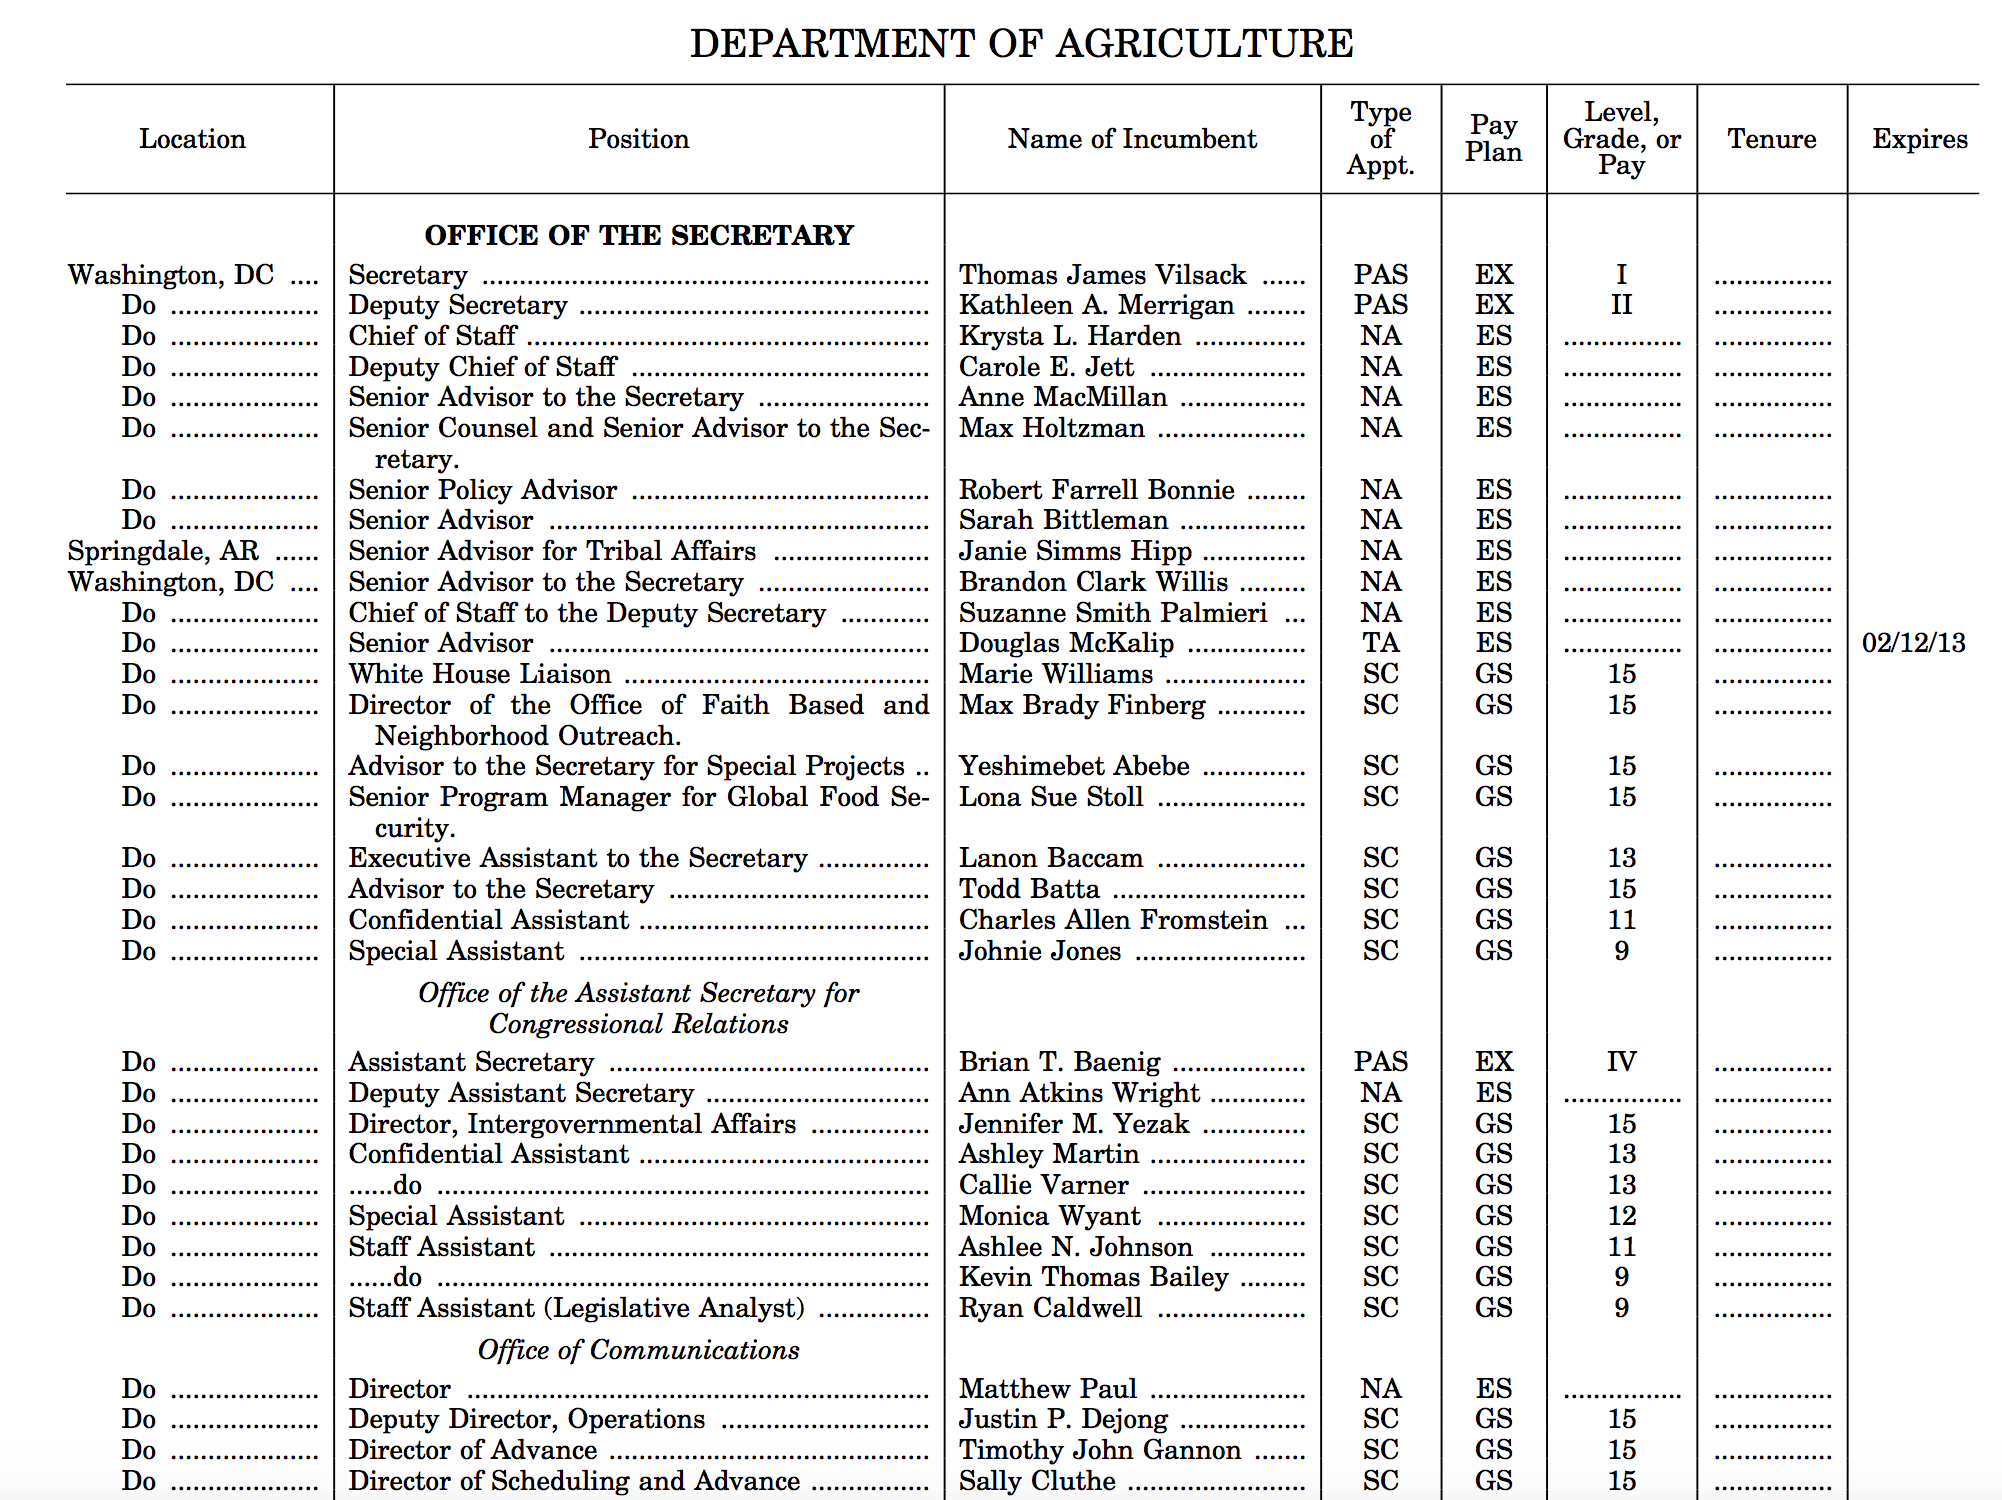
\includegraphics[height=5.5in,width=7in]{PlumBookPage.png}
\caption{Page from the Plum Book on the Department of Agriculture}
\end{center}
\end{figure}

\newpage
\begin{figure}[!htb]
\begin{center}
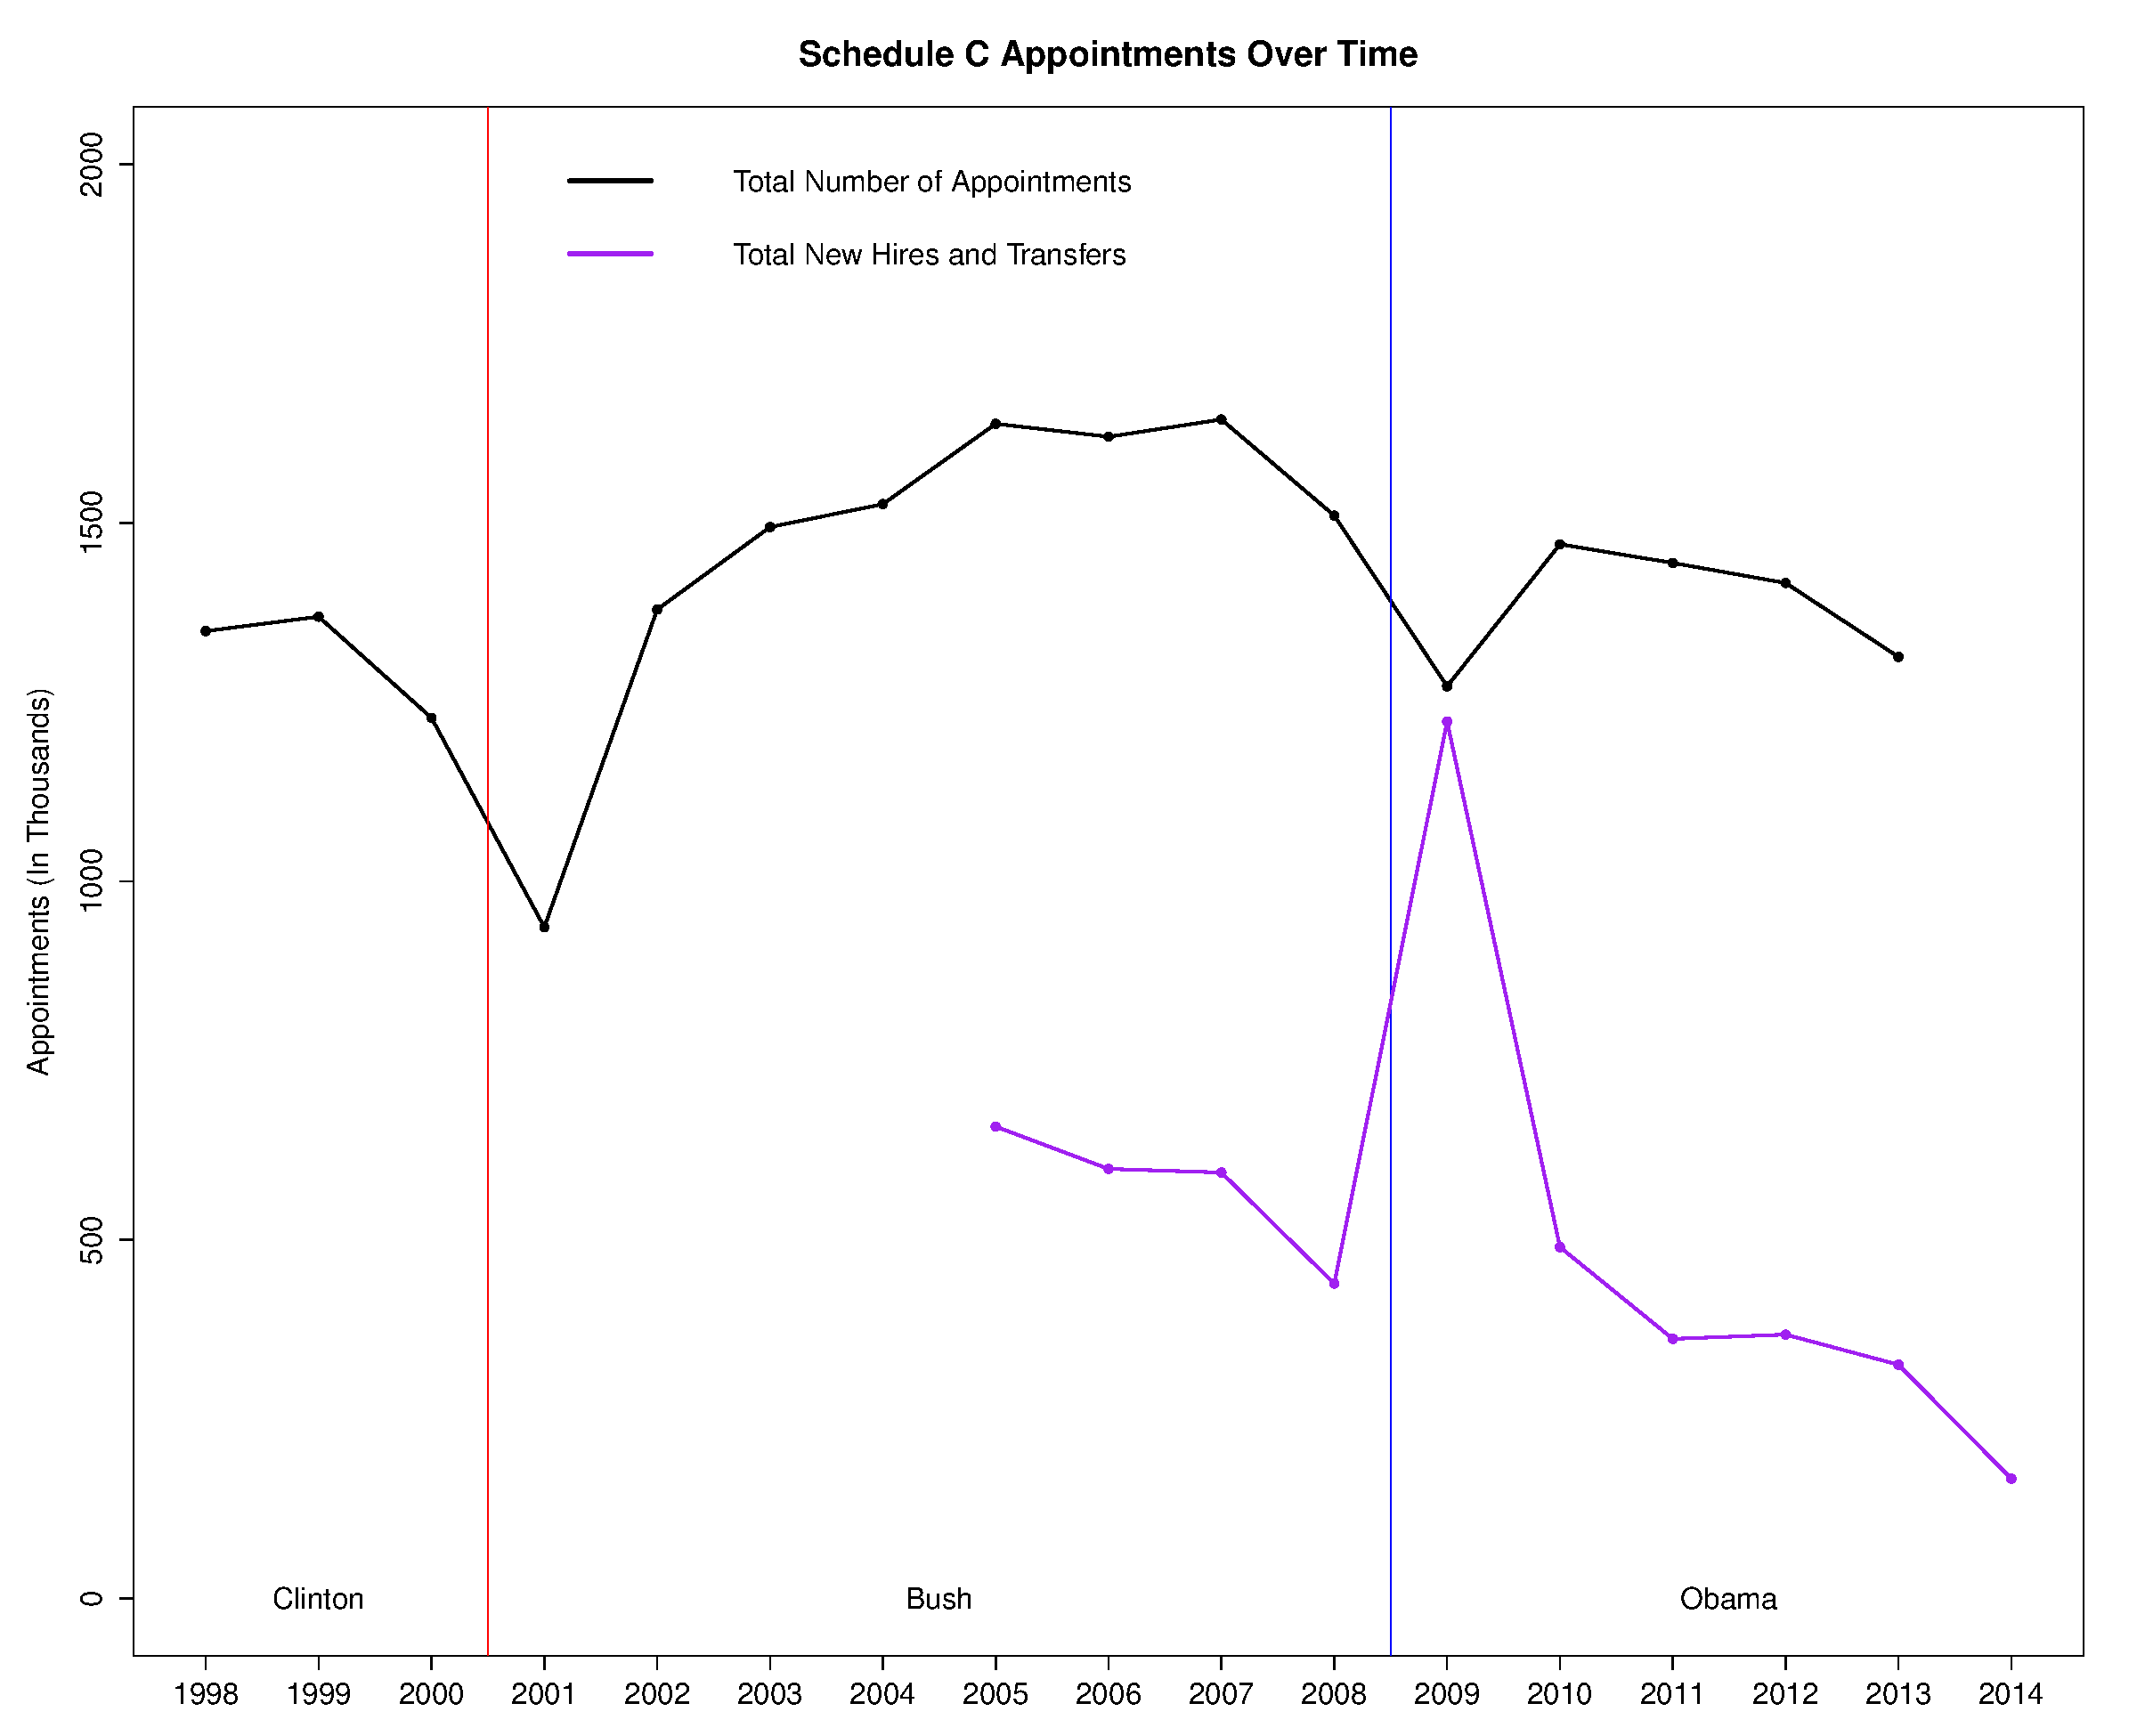
\includegraphics[height=5.5in,width=7in]{SCAptsandAccOverTime.pdf}
\caption{This plot shows the total number of Schedule C appointments over time (black line) in addition to the number of new hires and transfers added to the agency in a given year (purple line).}
\end{center}
\end{figure}

\newpage
\begin{figure}[!htb]
\begin{center}
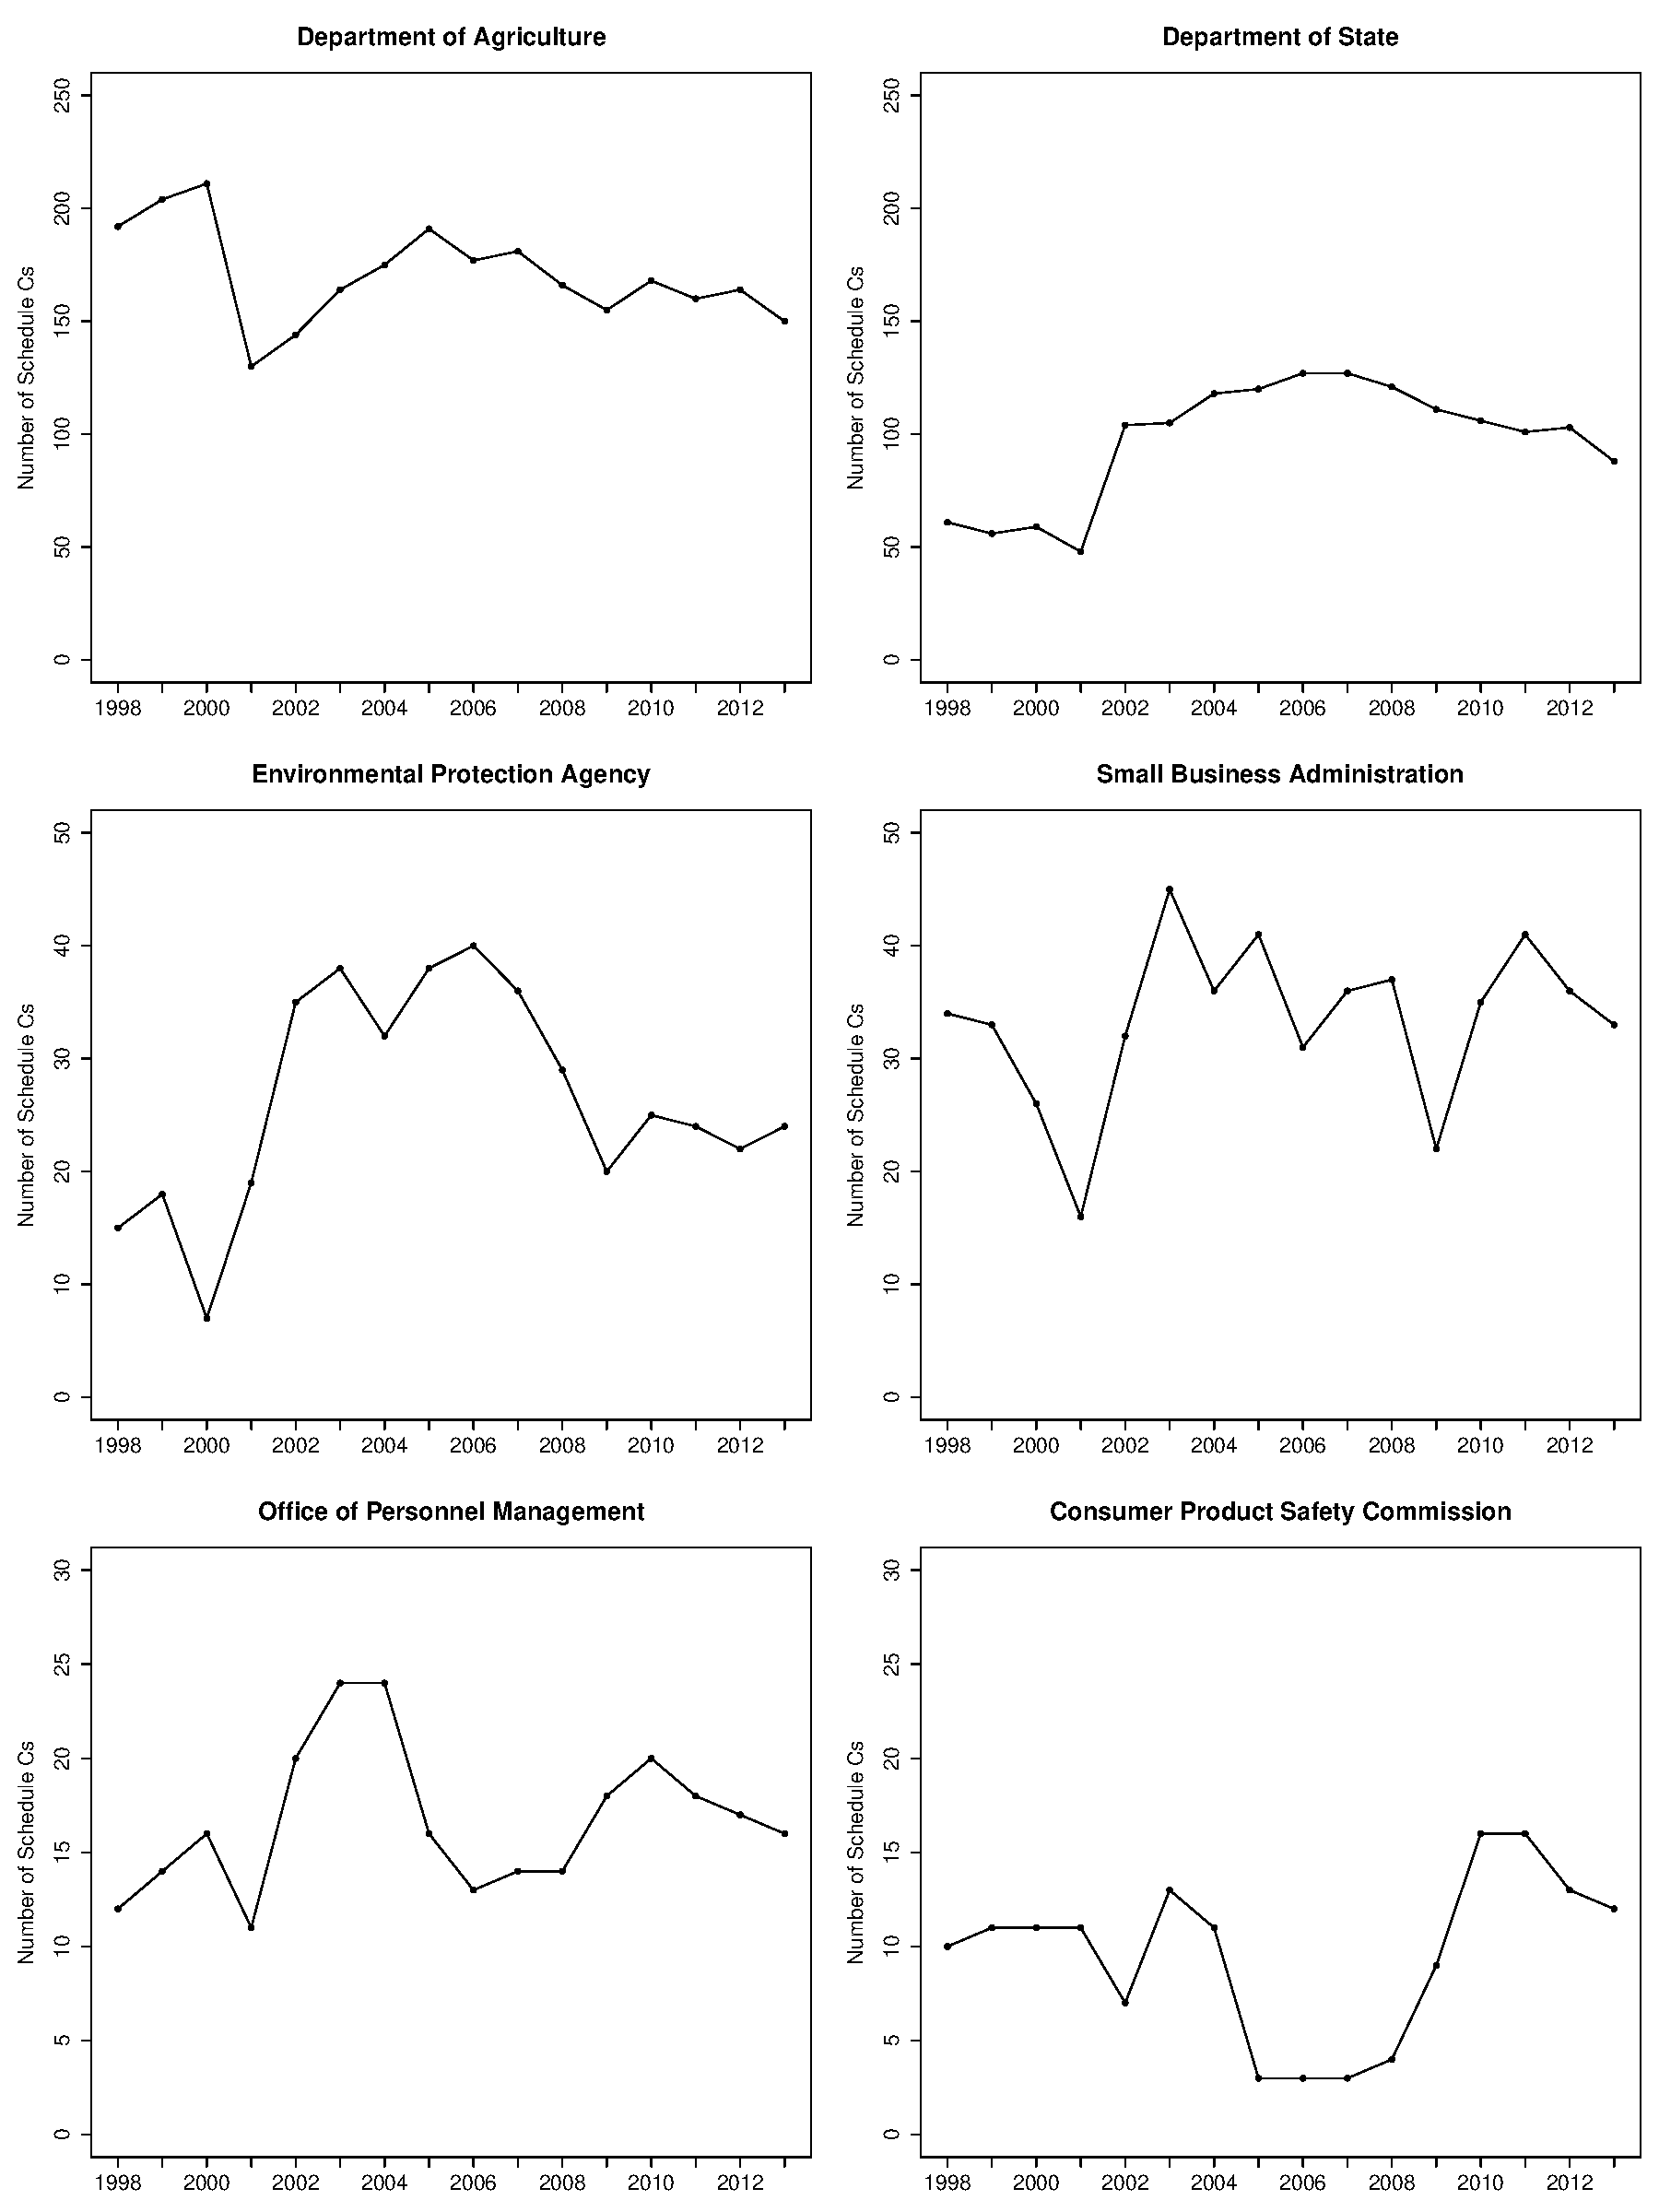
\includegraphics[height=8in,width=6in]{CountofSCsOverTimeSelectAgencies.pdf}
\caption{These plots show the number of Schedule C appointees over time in selected agencies.}
\end{center}
\end{figure}

\newpage
\begin{figure}[!h]
\begin{center}
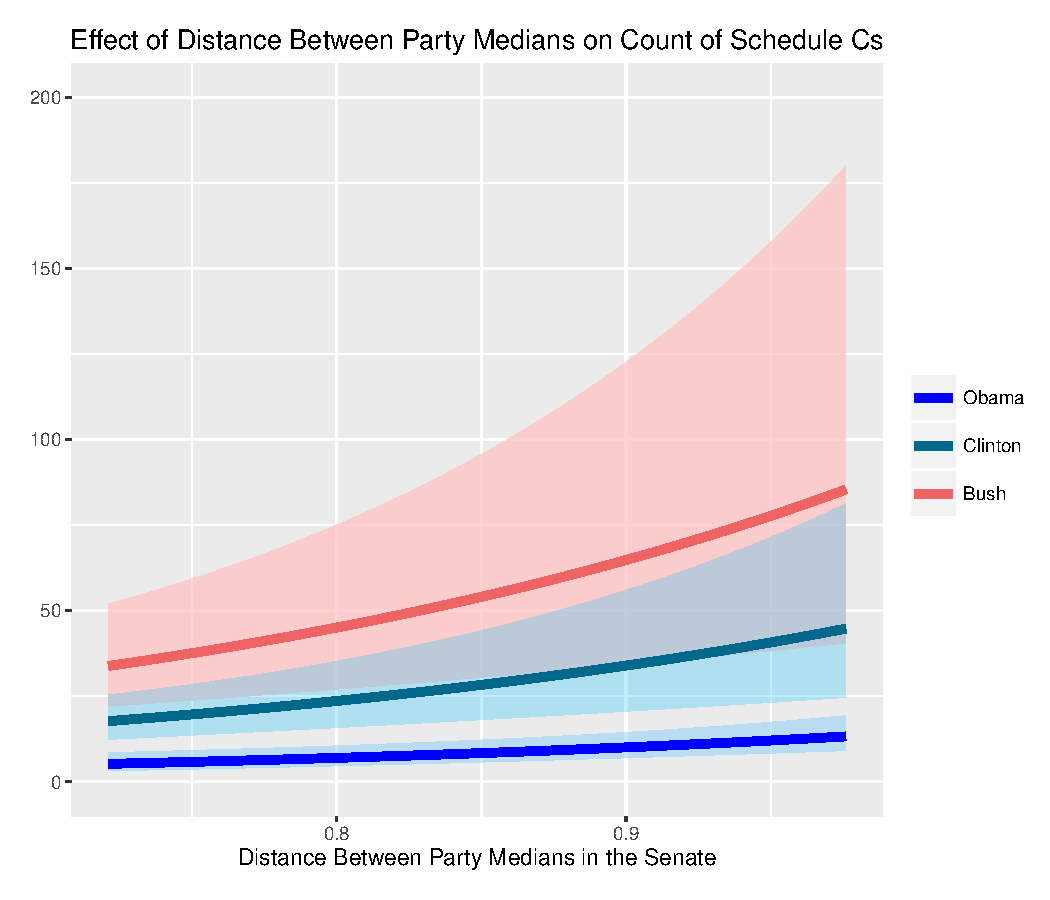
\includegraphics[height=4in,width=4.5in]{ResultsPlots.pdf}
\caption{Predicted Effect of the Ideological Distance Between Party Medians in the Senate on the Number of Schedule C Appointees in an Agency.}
\end{center}
\end{figure}

\newpage
\begin{figure}[!h]
\begin{center}
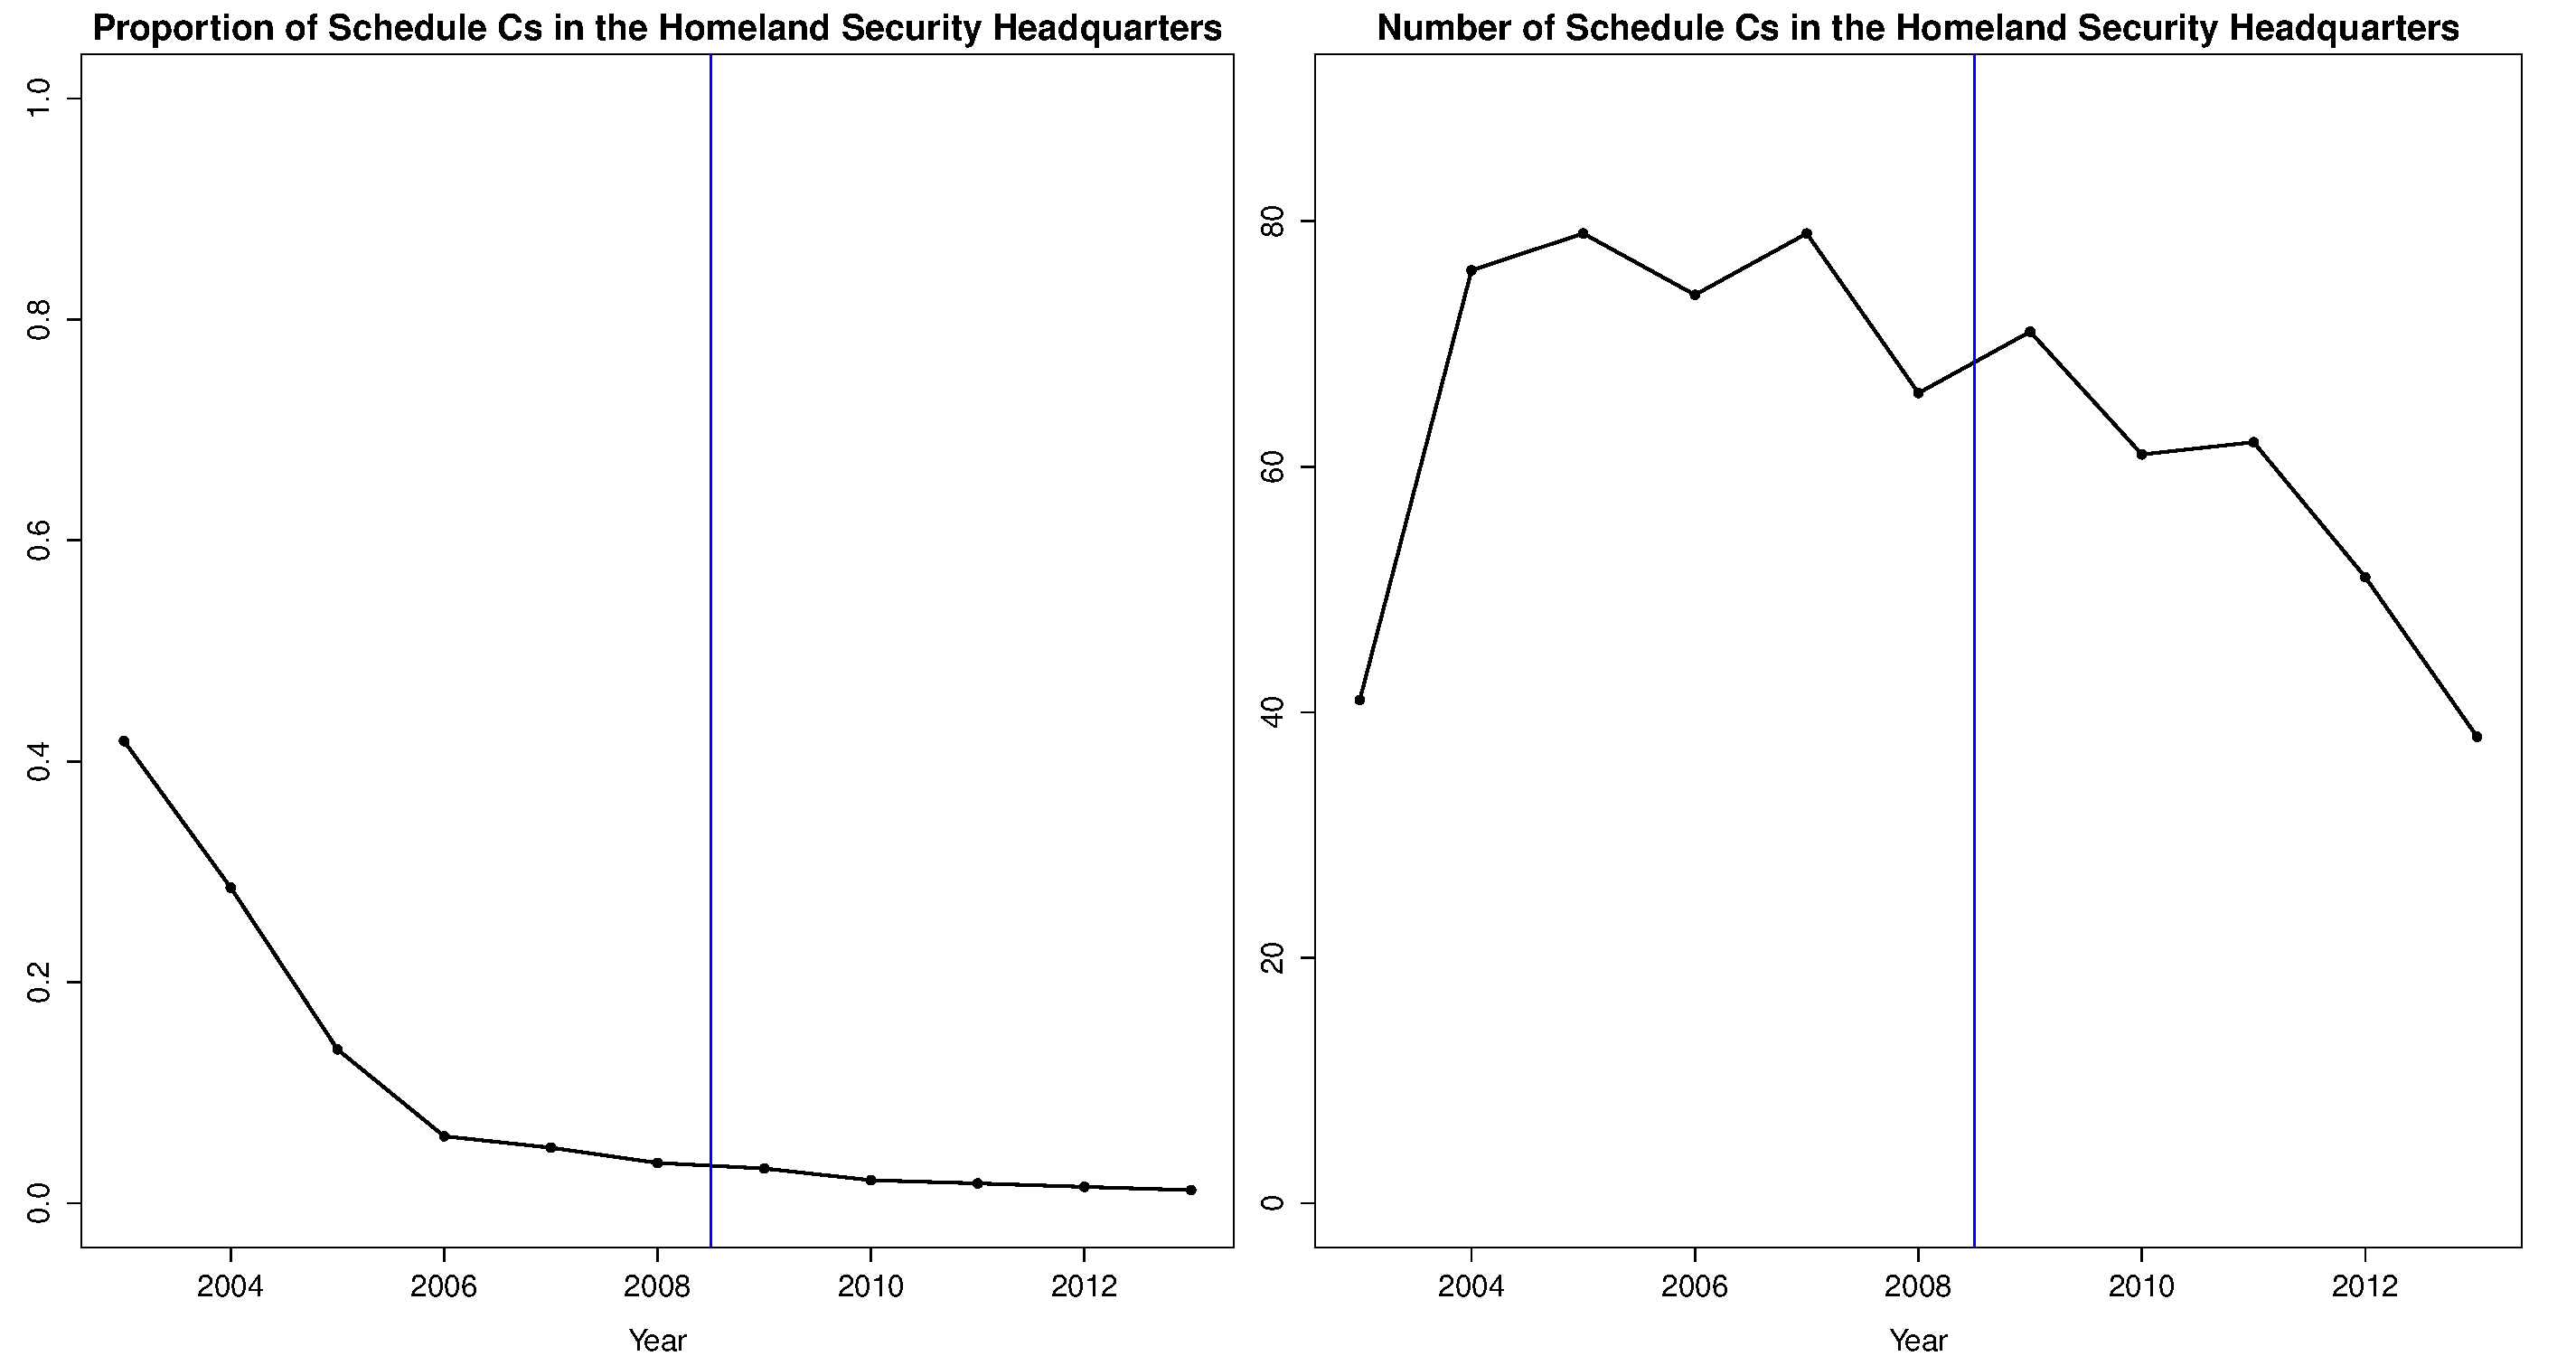
\includegraphics[height=3in,width=6in]{DHSProportionRawNumber.pdf}
\caption{Proportion and Raw Number of Schedule C and Excepted Service Executive Appointments in the Homeland Security Headquarters.}
\end{center}
\end{figure}

\newpage
\section*{Online Appendix: Alternative Model Specification}
\begin{table}[!htbp] \centering 
  \caption{Results Using Divided Government instead of Distance Between Party Medians} 
  \label{} 
\begin{tabular}{@{\extracolsep{5pt}}lcc} 
\\[-1.8ex]\hline 
\hline \\[-1.8ex] 
 & \multicolumn{2}{c}{\textit{Dependent variable: Count of Schedule Cs}} \\ 
\cline{2-3} 
\\[-1.8ex] & \multicolumn{2}{c}{ } \\ 
\\[-1.8ex] & (1) & (2)\\ 
\hline \\[-1.8ex] 
 Distance Agency to President & $-$2.472$^{*}$ & $-$2.442$^{*}$ \\ 
  & (0.440) & (0.430) \\ 
  & & \\ 
 Divided Government& 0.213$^{*}$ & 0.153$^{*}$ \\ 
  & (0.053) & (0.039) \\ 
  & & \\ 
 Distance President 60th Senator & $-$1.329$^{*}$ &  \\ 
  & (0.310) &  \\ 
  & & \\ 
 Size (Thousands) & 0.009$^{*}$ & 0.009$^{*}$ \\ 
  & (0.002) & (0.002) \\ 
  & & \\ 
 First Year of Presidency & $-$0.388$^{*}$ & $-$0.299$^{*}$ \\ 
  & (0.063) & (0.053) \\ 
  & & \\ 
 Last Year of Presidency & $-$0.023 & $-$0.001 \\ 
  & (0.020) & (0.023) \\ 
  & & \\ 
 Obama & $-$1.430$^{*}$ & $-$1.136$^{*}$ \\ 
  & (0.247) & (0.216) \\ 
  & & \\ 
 Clinton & $-$0.998$^{*}$ & $-$0.881$^{*}$ \\ 
  & (0.245) & (0.227) \\ 
  & & \\ 
 Constant & 5.400$^{*}$ & 4.338$^{*}$ \\ 
  & (0.571) & (0.400) \\ 
  & & \\ 
\hline \\[-1.8ex] 
\hline 
\hline \\[-1.8ex] 
\textit{Note:}  & \multicolumn{2}{r}{$^{*}$p$<$0.05} \\ 
\end{tabular} 
\end{table}

\newpage
\section*{Online Appendix: Histogram of Counts of Schedule Cs.}
\begin{figure}[!h]
\begin{center}
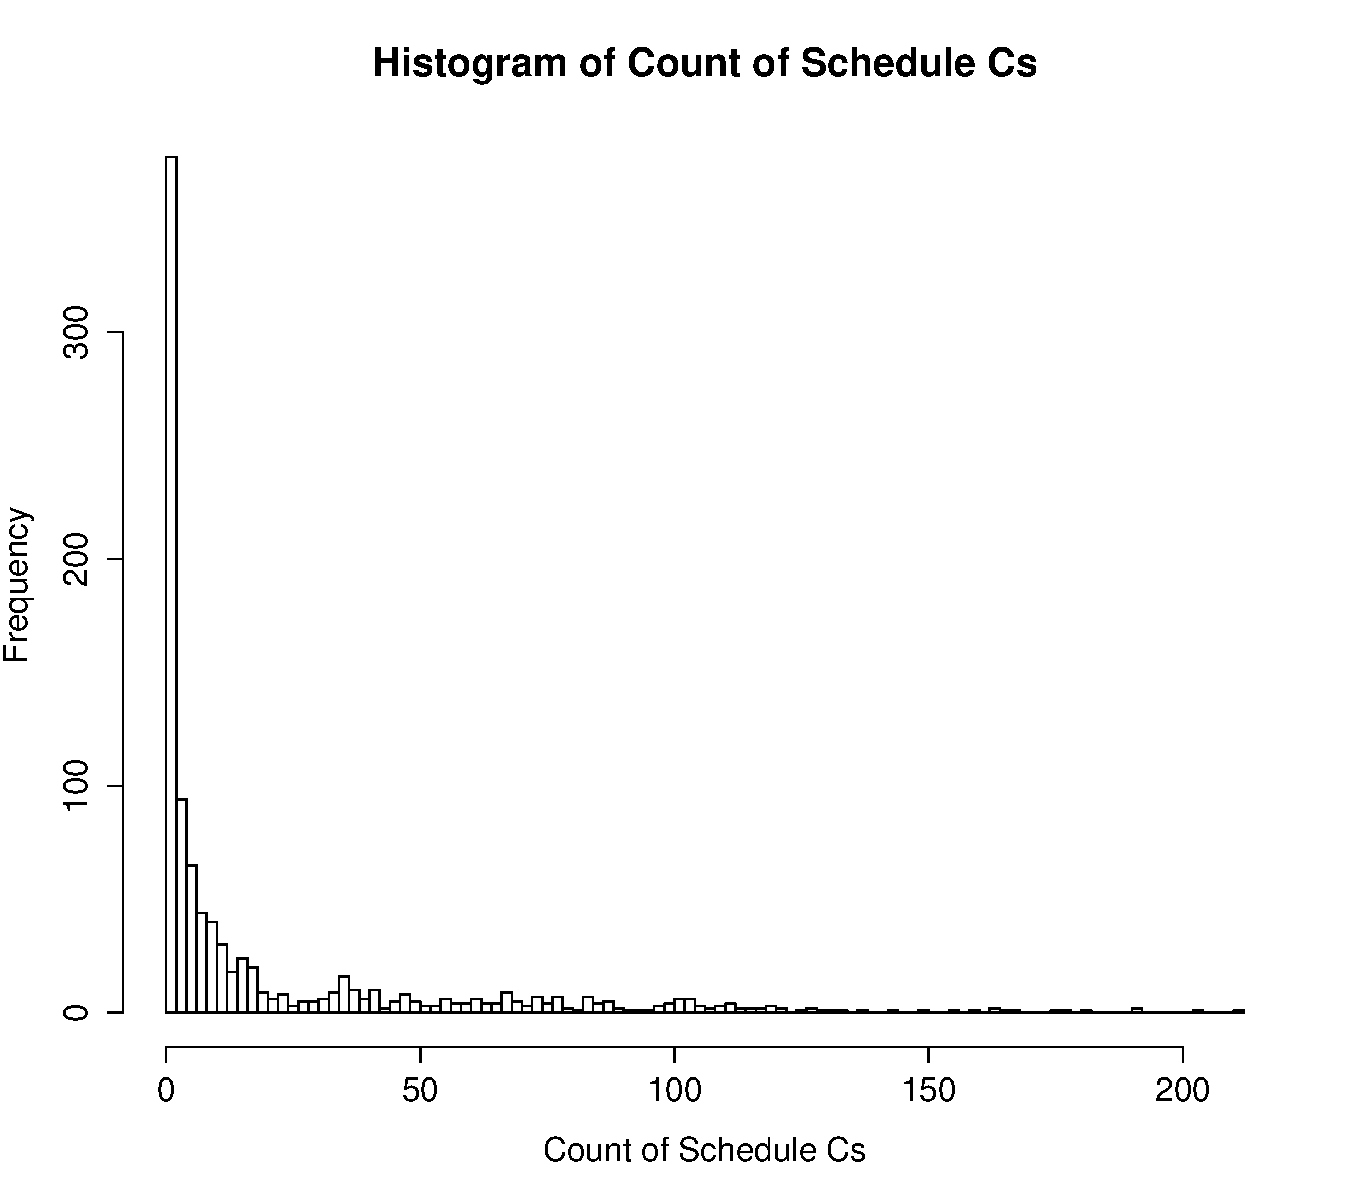
\includegraphics[height=4in,width=5in]{HistogramScheduleCCount.pdf}
\caption{Histogram of Number of Schedule Cs in Agencies.}
\end{center}
\end{figure}




	
%Cooney story	
%	If there is any doubt left over the importance of excepted positions, consider the 2005 Cooney scandal in the Council on Environmental Quality (CEQ). The CEQ formulates reports about the status of environmental resources, reviews the environmental activities of governmental and non-governmental organizations, and oversees the implementation of the environmental impact assessment process. While the CEQ is theoretically designed such that environmental experts assess environmental impact, in reality, the process is often political. Phillip Cooney, who served in an excepted position as CEQ Chief of Staff, had only one qualification relating to the job: he had been employed as a lobbyist for the American Petroleum Institute. In 2005, a scandal broke from a report showing that Cooney purposefully doctored expert-prepared government climate reports to downplay scientific climate change findings. One anonymous EPA employee noted that, for many, Cooney's editing had damaged morale and ``created a sense of frustration'' (Revkin 2005a). The Cooney example exemplifies both the importance of excepted appointments as a political tool to advance the president's interests and the power they are able to wield over policies. 

%Miscellaneous sentences to put in other places:

%It would be easy to conclude that PAS appointees are the only bureaucrats deserving of attention. After all, there is often considerable speculation and controversy surrounding confirmation battles, and these personnel serve in some of the most important positions as cabinet secretaries and heads of independent agencies. 


\end{document}
